\chapter*{Huaraz, Cordillera Blanca et Trujillo\markboth{Huaraz, Cordillera Blanca et Trujillo}{}}
\section*{13 juin 2015}

Huaraz est située à environ 3000m d'altitude au coeur de la Cordillera Blanca, chaîne de montagnes avec plusieurs sommets à plus de 6000m dont le fameux Mont Huascaran. 
\begin{center} 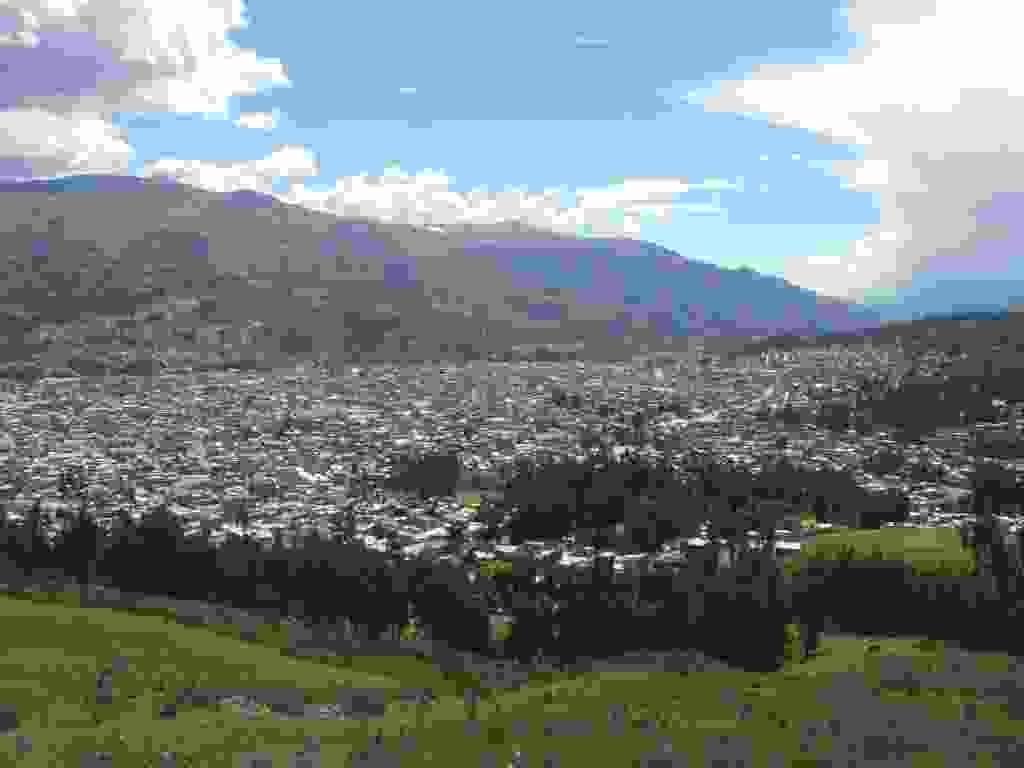
\includegraphics[width=\mywidth]{../wp-content/uploads/2015/06/P6034650-1024x768.jpg} \end{center}
\begin{center} 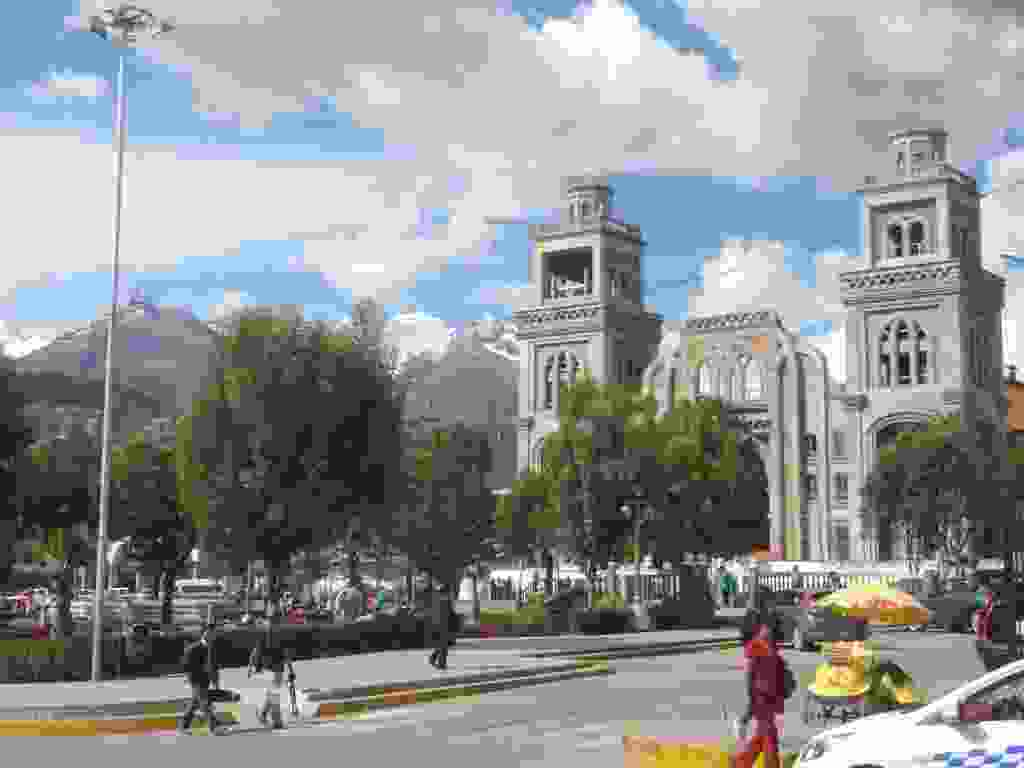
\includegraphics[width=\mywidth]{../wp-content/uploads/2015/06/P6034653-1024x768.jpg} \end{center}

Marché d'Huaraz : 
\begin{center} 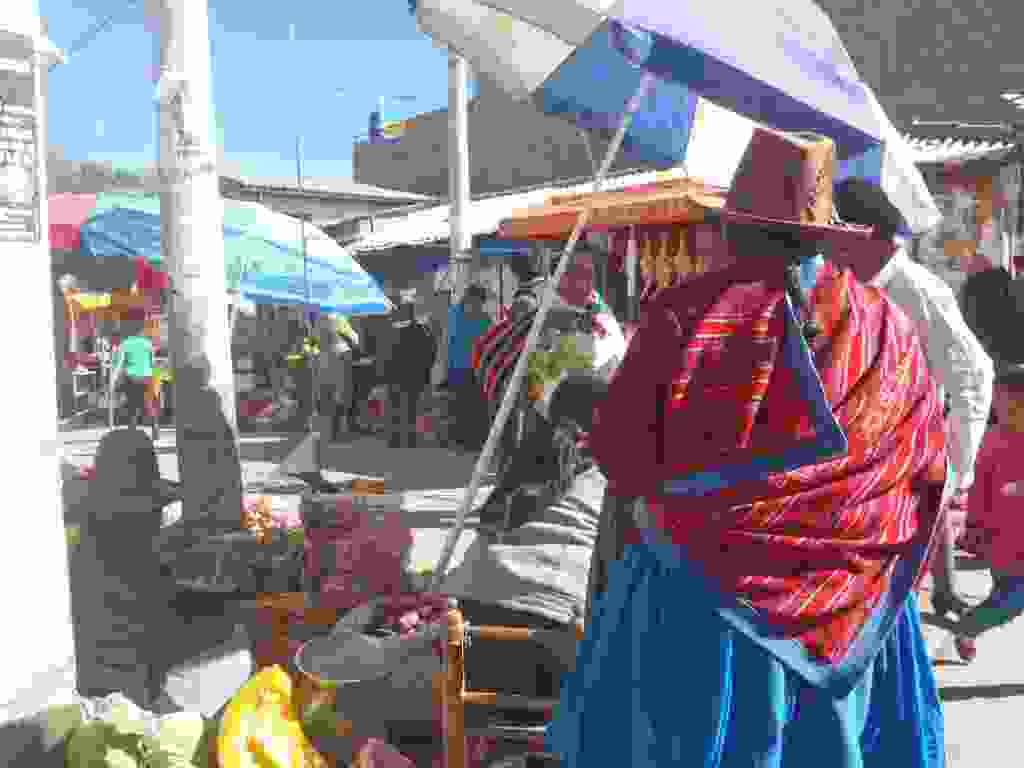
\includegraphics[width=\mywidth]{../wp-content/uploads/2015/06/P6034638-1024x768.jpg} \end{center}
\begin{center} 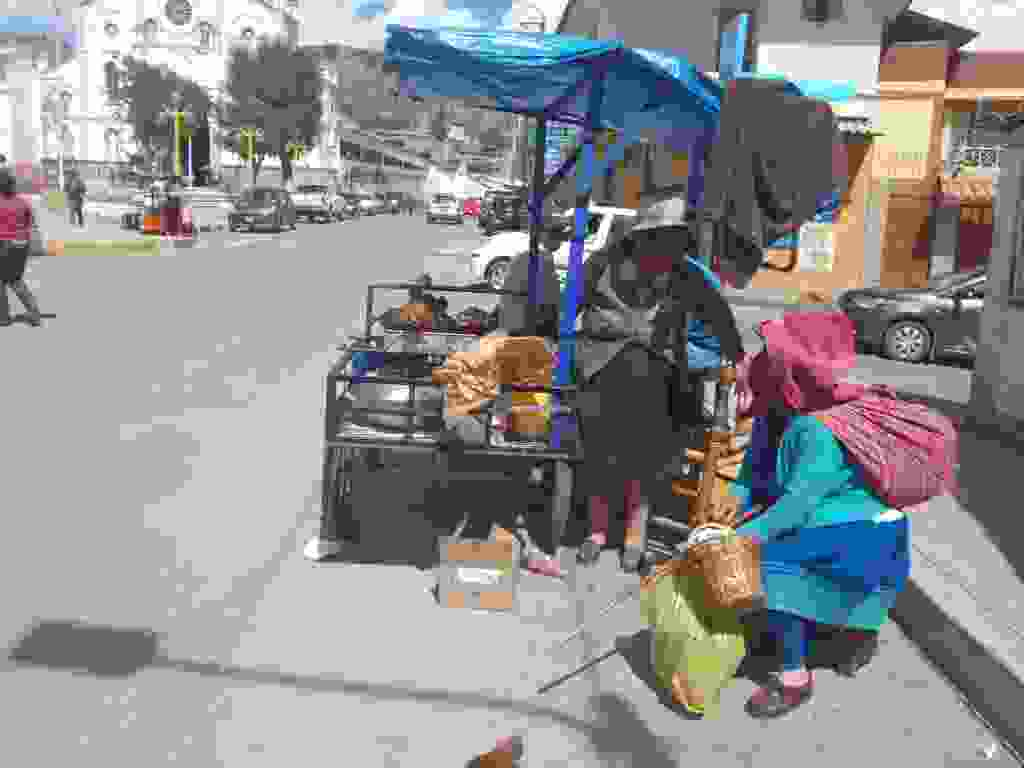
\includegraphics[width=\mywidth]{../wp-content/uploads/2015/06/P6034642-1024x768.jpg} \end{center}

J'aurais bien tenté un sommet dans le parc national Huascaran, mais le temps qui me reste jusqu'en Equateur et le prix des ascensions m'en ont dissuadés. 
À la place j'ai fait 2 randonnées à la journée : 
d'abord juste au dessus d'Huaraz pour aller voir la Laguna Churup. 
\begin{center} 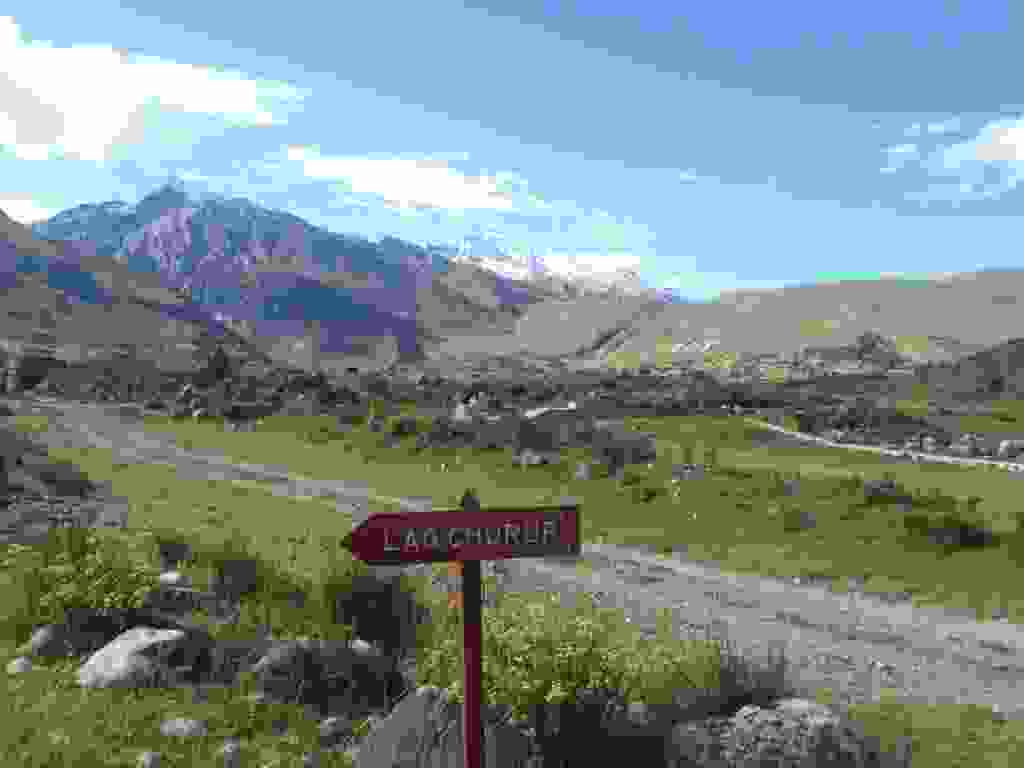
\includegraphics[width=\mywidth]{../wp-content/uploads/2015/06/P6044656-1024x768.jpg} \end{center}
\begin{center} 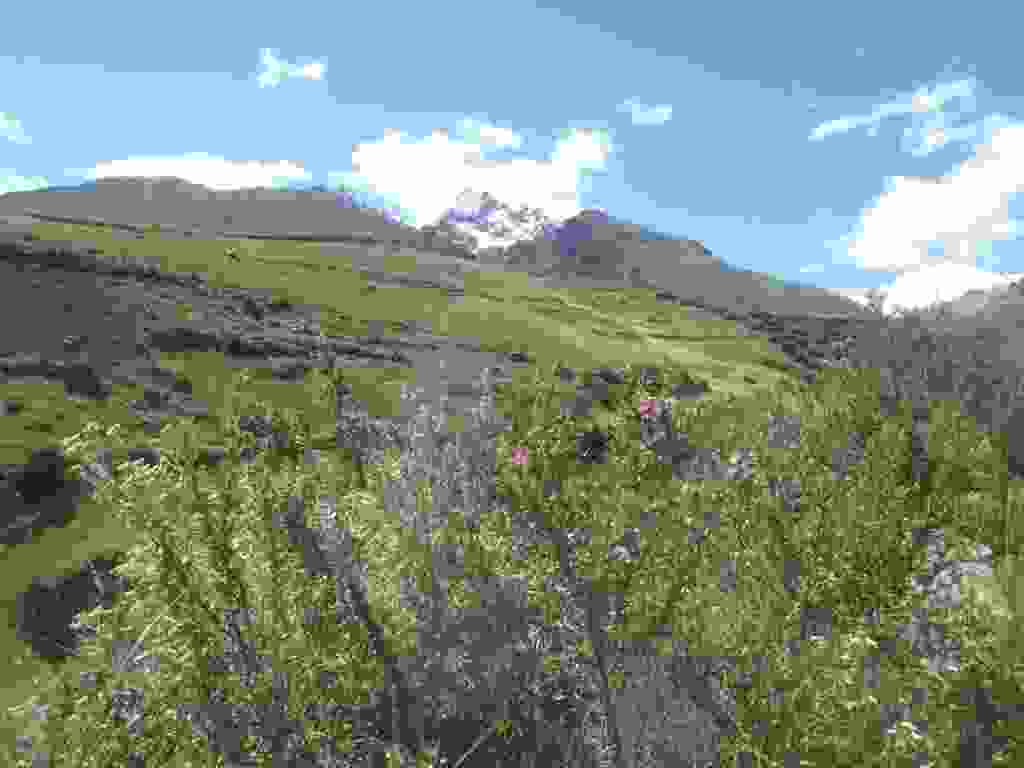
\includegraphics[width=\mywidth]{../wp-content/uploads/2015/06/P6044679-1024x768.jpg} \end{center}
\begin{center} 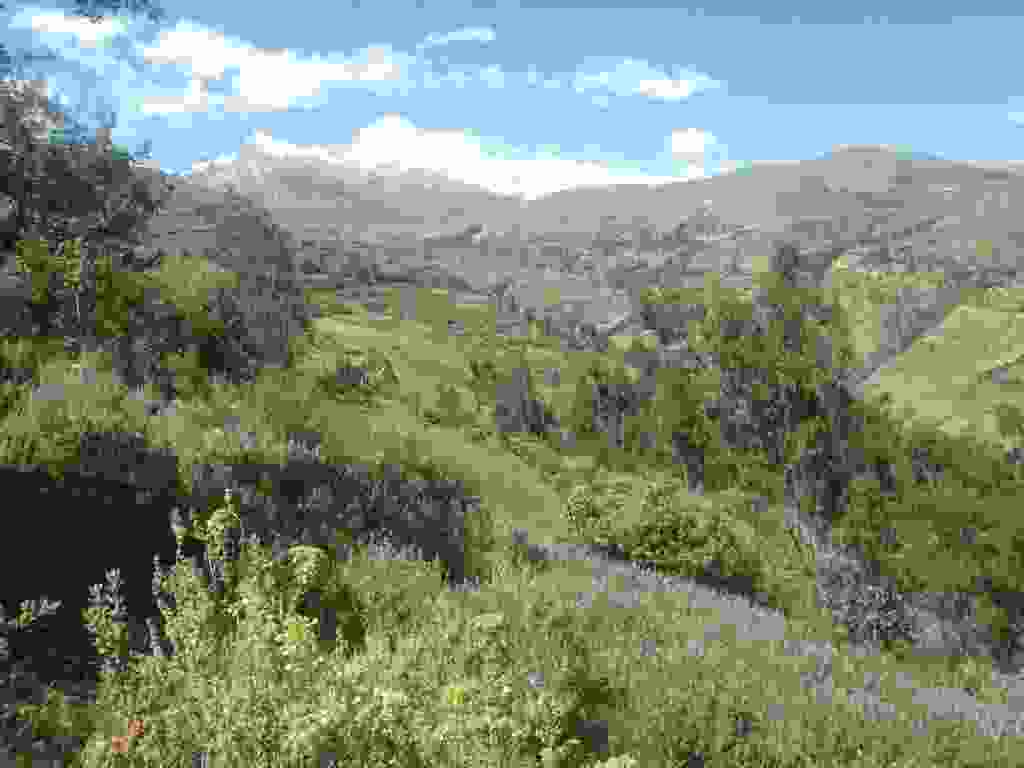
\includegraphics[width=\mywidth]{../wp-content/uploads/2015/06/P6044681-1024x768.jpg} \end{center}
\begin{center} 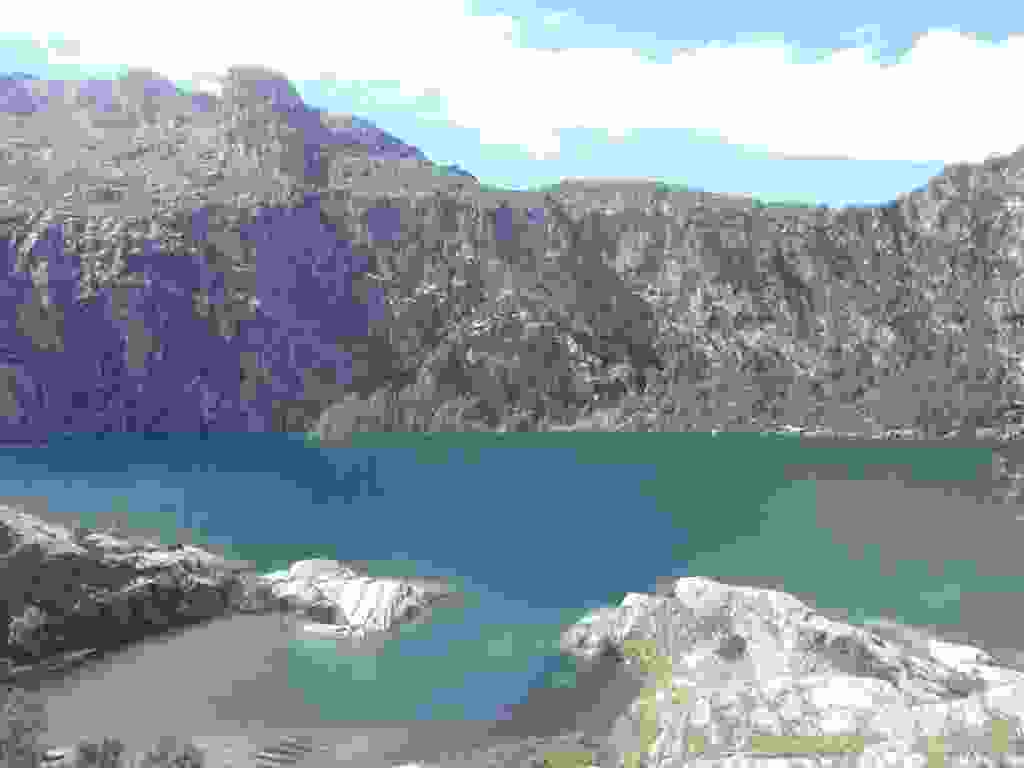
\includegraphics[width=\mywidth]{../wp-content/uploads/2015/06/P6044670-1024x768.jpg} \end{center}
\begin{center} 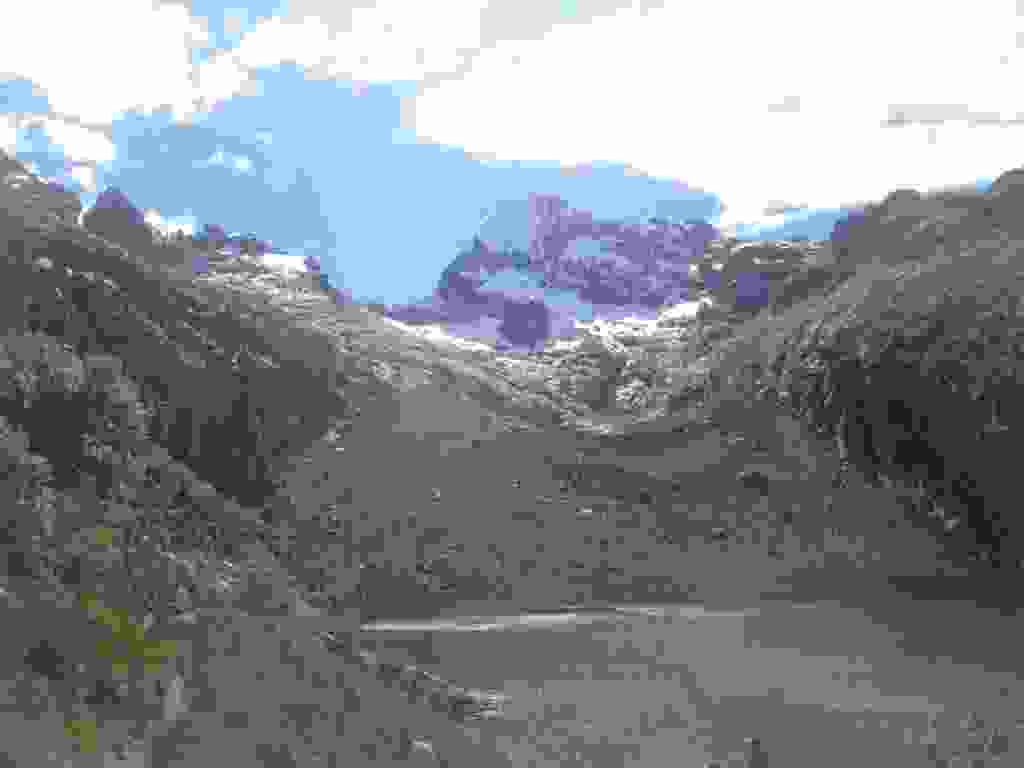
\includegraphics[width=\mywidth]{../wp-content/uploads/2015/06/P6044674-1024x768.jpg} \end{center}

\pagebreak
Puis une journée de vélo plus loin, la Laguna 69. J'ai fait la rando avec Elise et Laurent, cyclistes rencontrés le matin. 
\begin{center} 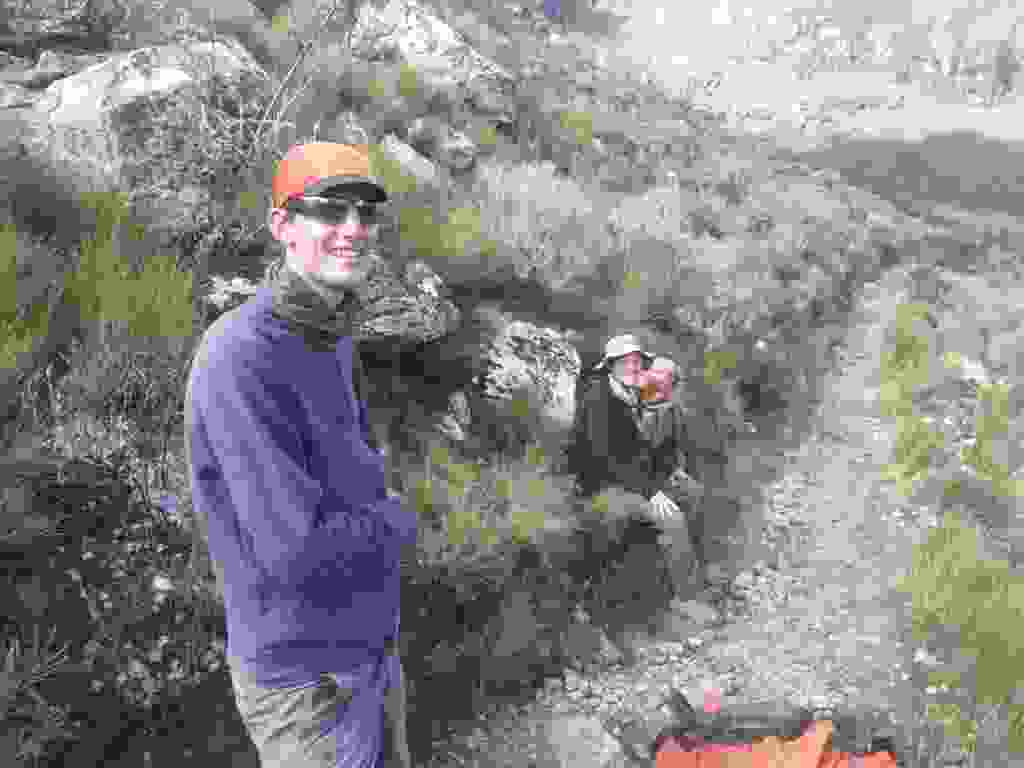
\includegraphics[width=\mywidth]{../wp-content/uploads/2015/06/P6064713-1024x768.jpg} \end{center}
\begin{center} 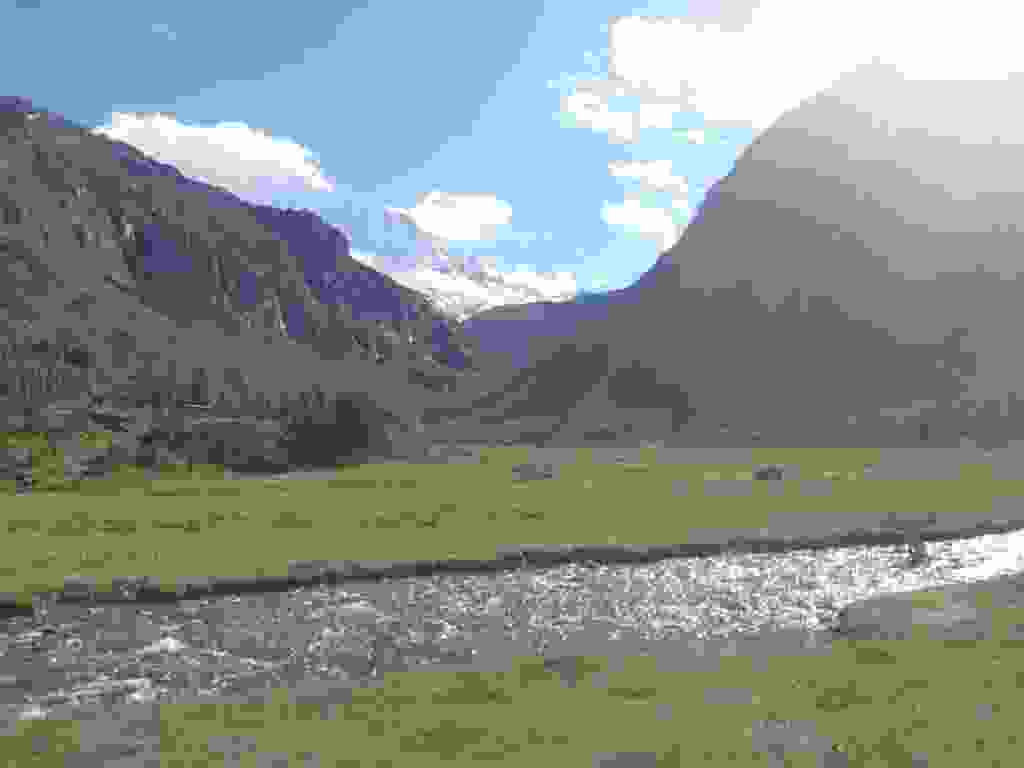
\includegraphics[width=\mywidth]{../wp-content/uploads/2015/06/P6064706-1024x768.jpg} \end{center}
\begin{center} 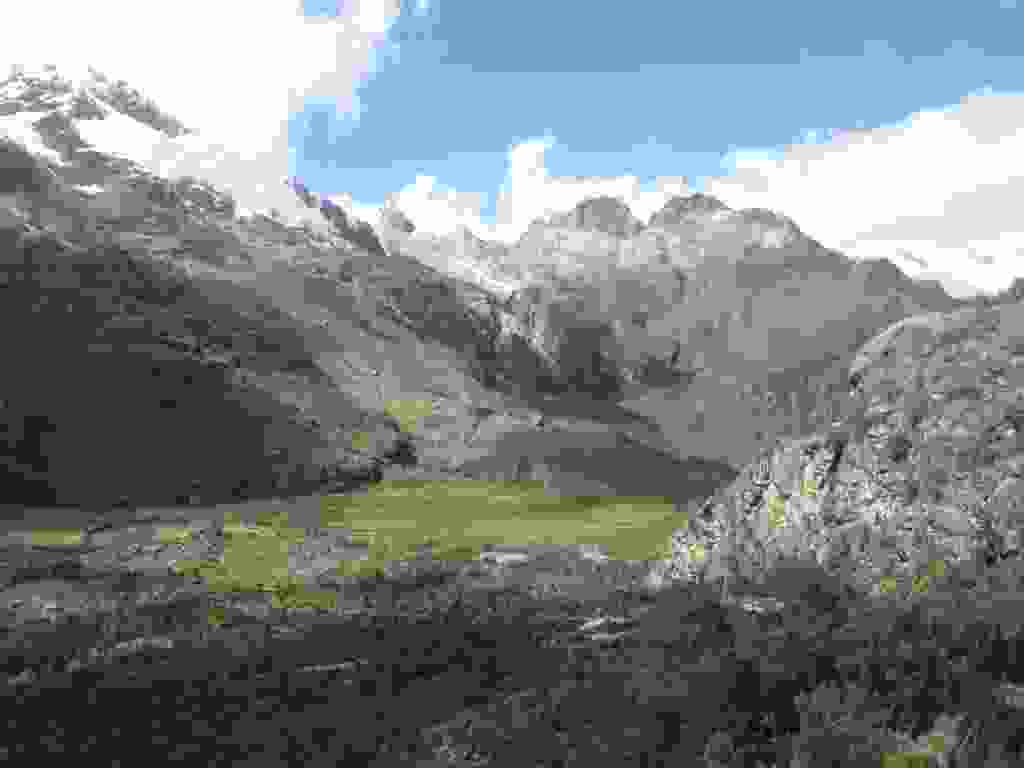
\includegraphics[width=\mywidth]{../wp-content/uploads/2015/06/P6064719-1024x768.jpg} \end{center}
\begin{center} 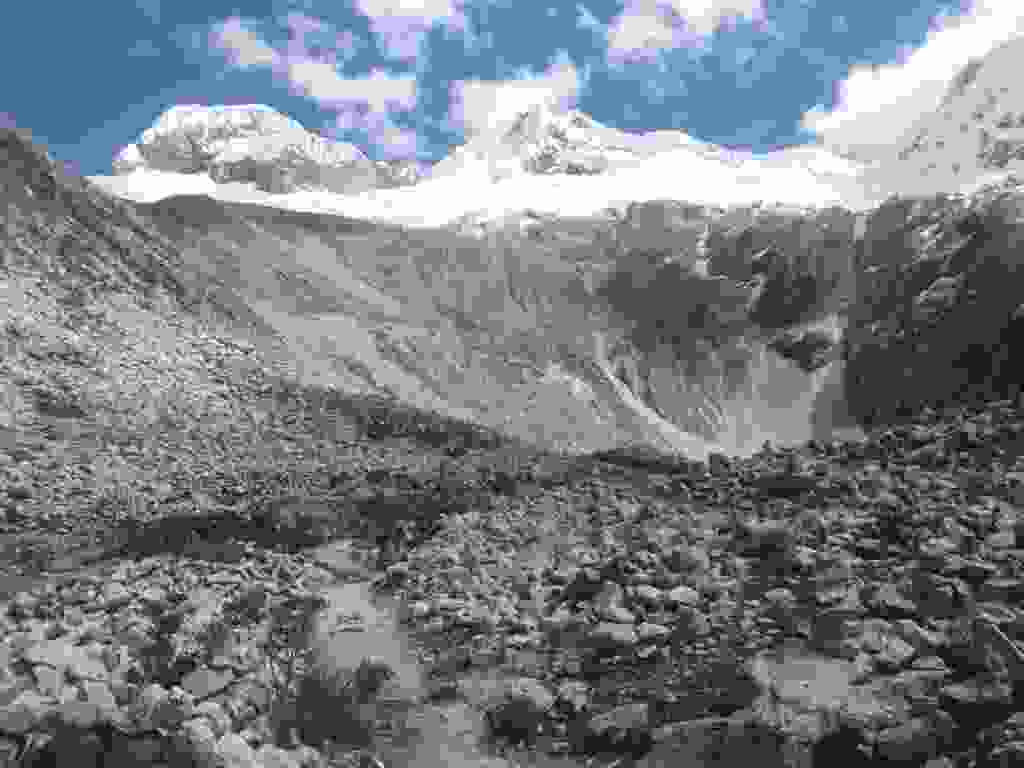
\includegraphics[width=\mywidth]{../wp-content/uploads/2015/06/P6064720-1024x768.jpg} \end{center}
\begin{center} 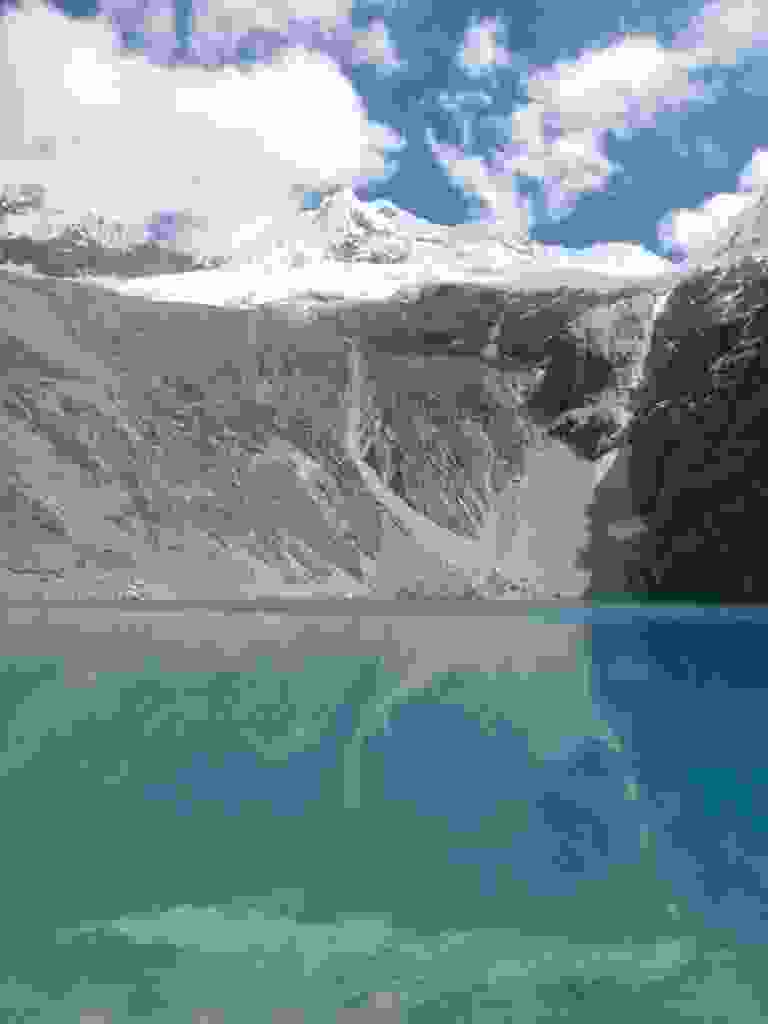
\includegraphics[height=\mywidth]{../wp-content/uploads/2015/06/P6064726-768x1024.jpg} \end{center}
\begin{center} 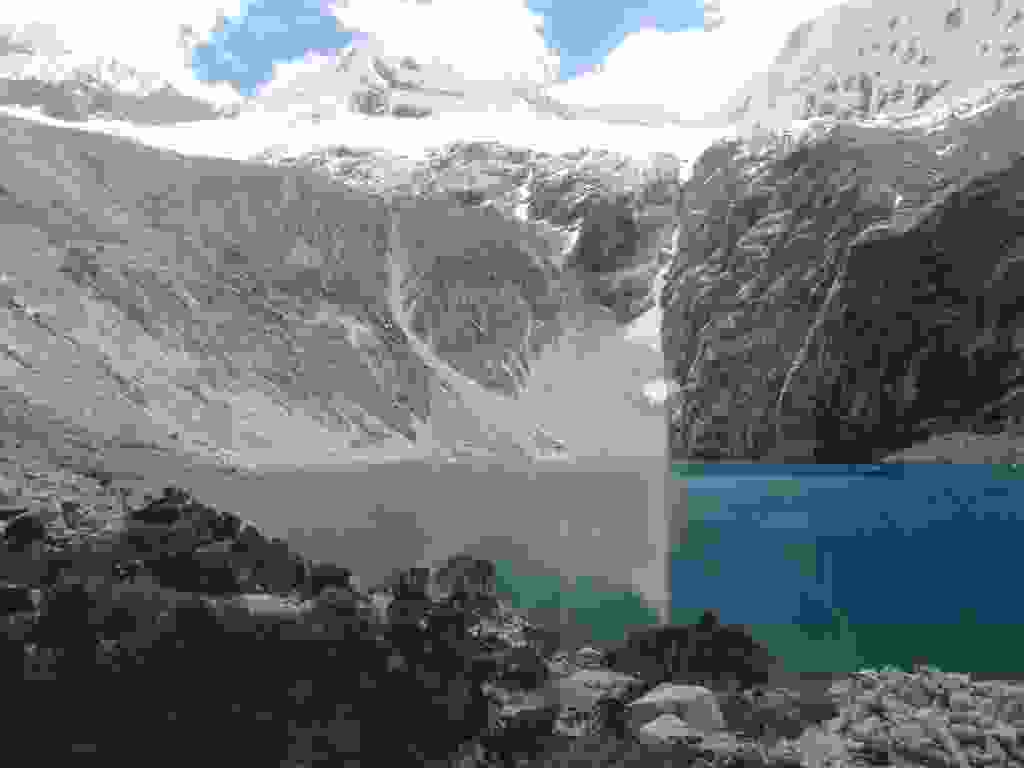
\includegraphics[width=\mywidth]{../wp-content/uploads/2015/06/P6064733-1024x768.jpg} \end{center}
\begin{center} 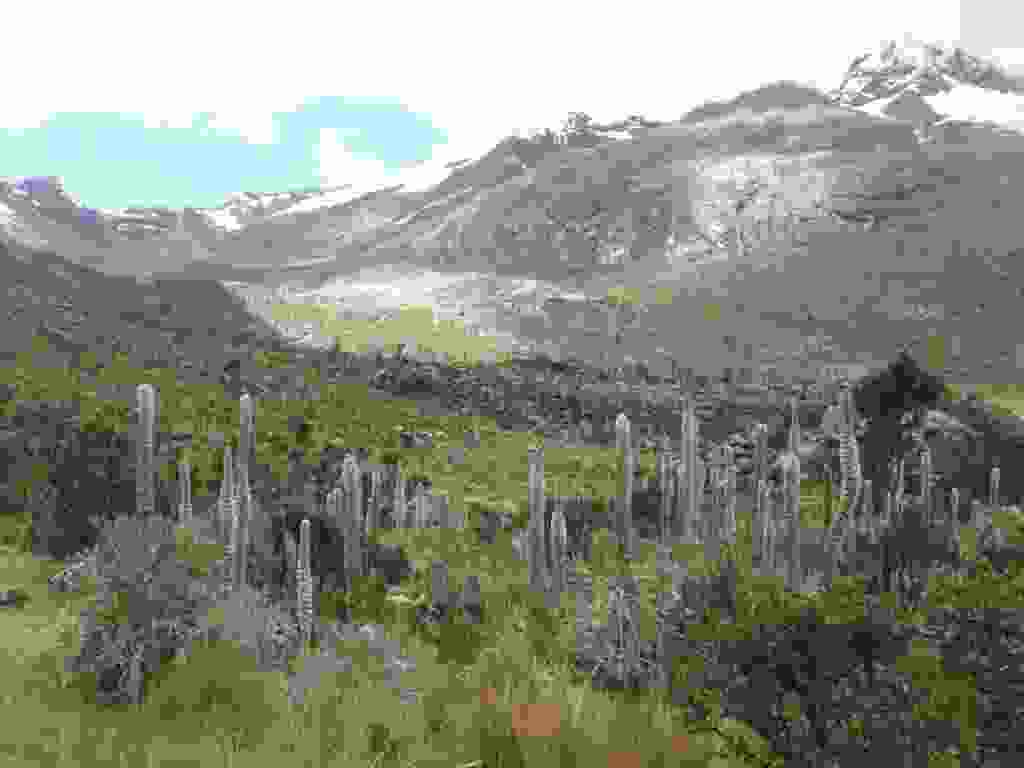
\includegraphics[width=\mywidth]{../wp-content/uploads/2015/06/P6064739-1024x768.jpg} \end{center}
\begin{center} 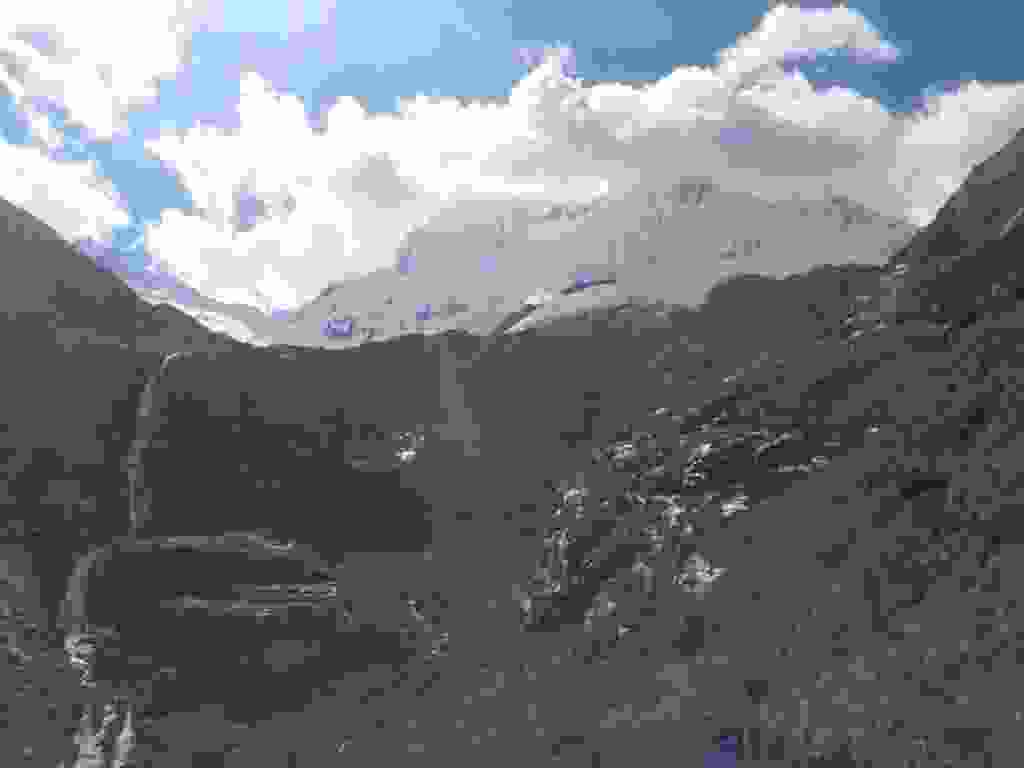
\includegraphics[width=\mywidth]{../wp-content/uploads/2015/06/P6064743-1024x768.jpg} \end{center}
\begin{center} 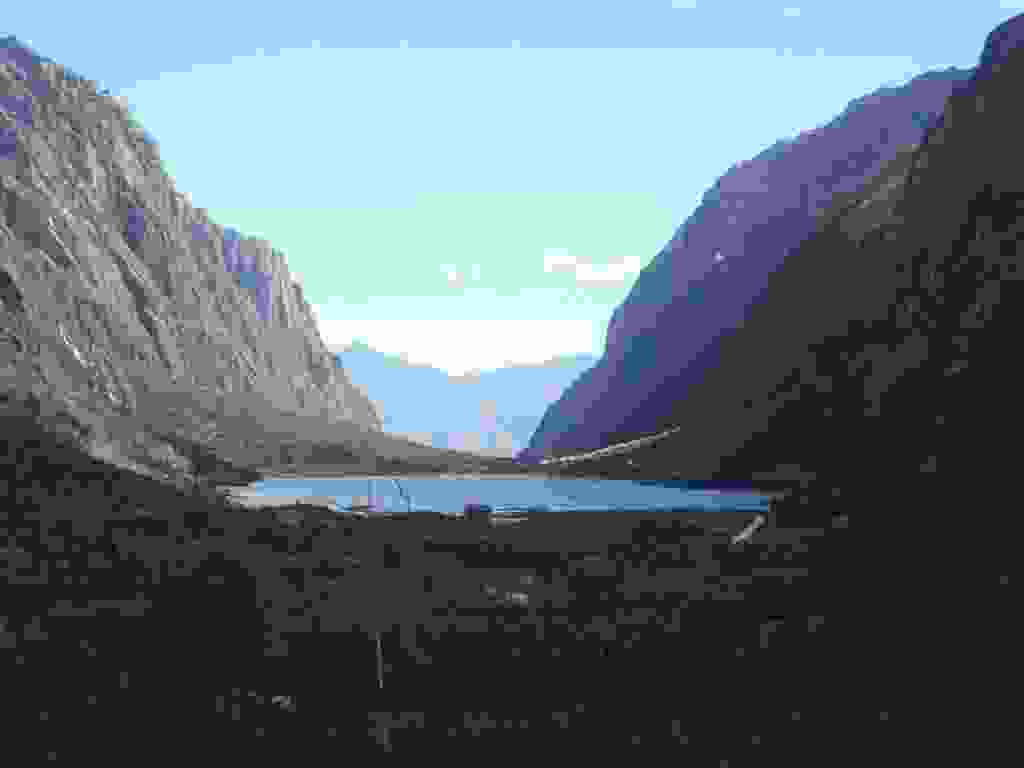
\includegraphics[width=\mywidth]{../wp-content/uploads/2015/06/P6064745-1024x768.jpg} \end{center}

J'ai ensuite repris le vélo sur la route qui longe la Cordillera Blanca. J´y ai croisé quelques voyageurs à vélo et à moto. 
\begin{center} 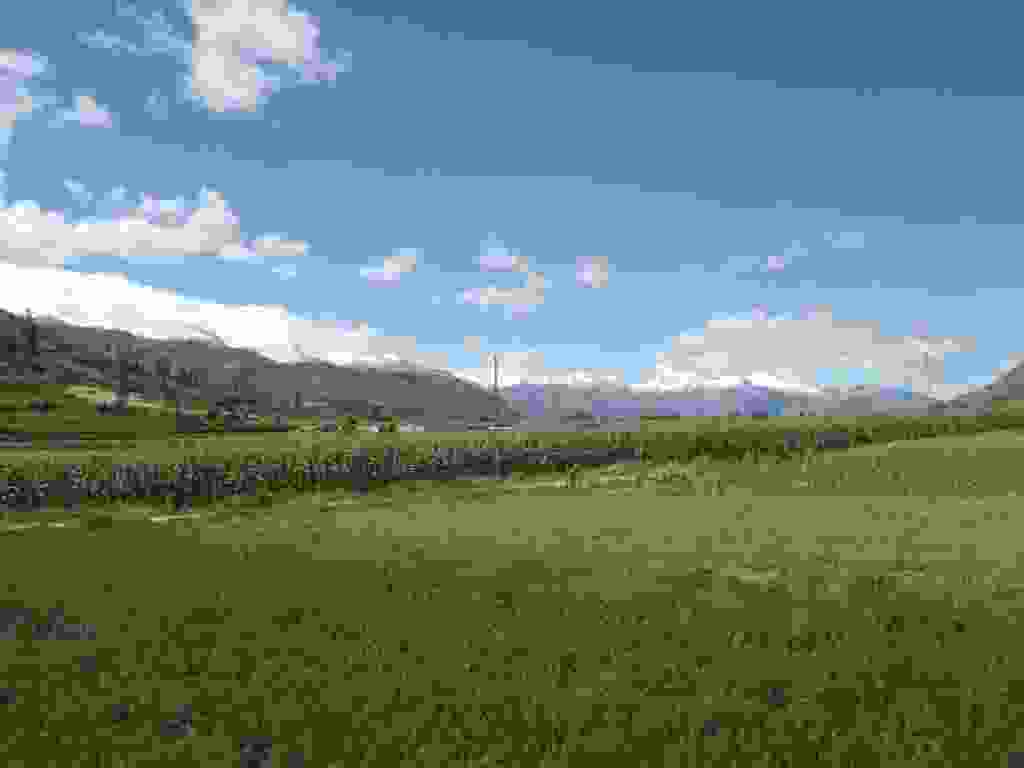
\includegraphics[width=\mywidth]{../wp-content/uploads/2015/06/P6054697-1024x768.jpg} \end{center}
\begin{center} 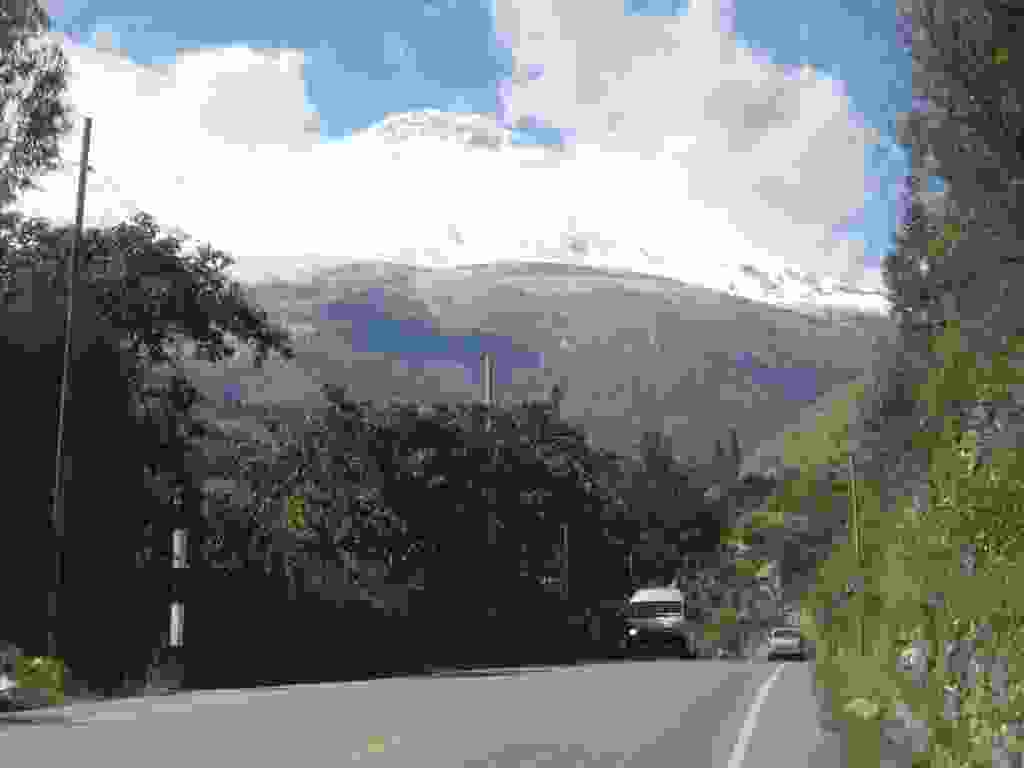
\includegraphics[width=\mywidth]{../wp-content/uploads/2015/06/P6054699-1024x768.jpg} \end{center}
\begin{center} 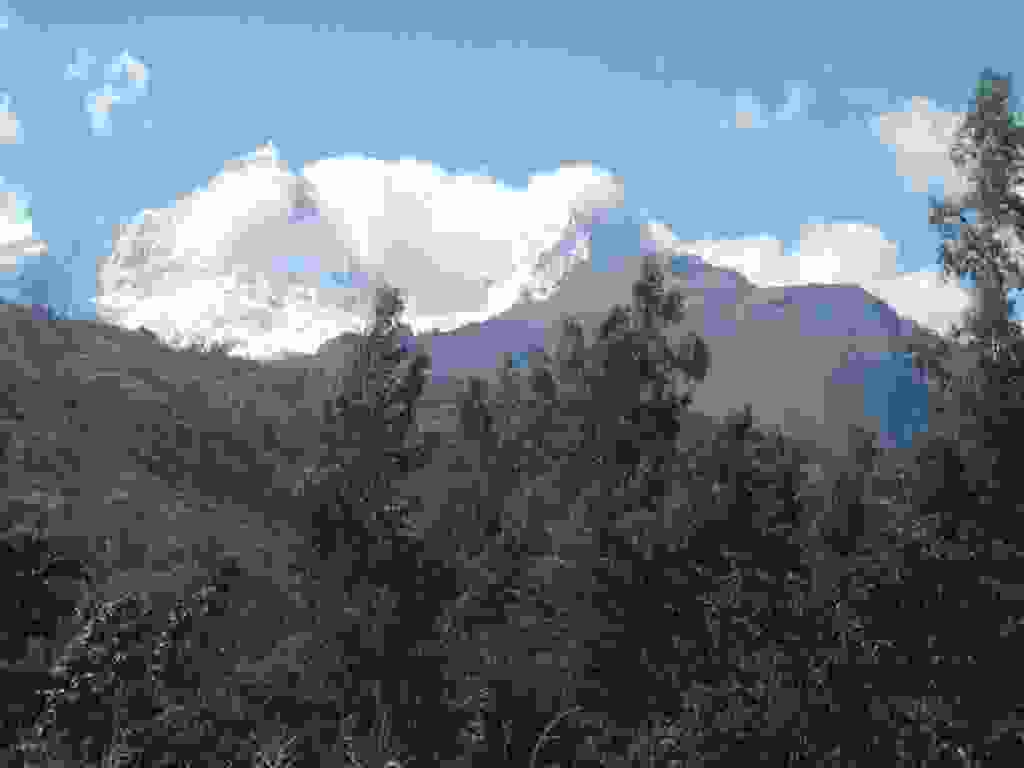
\includegraphics[width=\mywidth]{../wp-content/uploads/2015/06/P6054701-1024x768.jpg} \end{center}

\pagebreak
Ensuite descente du canyon del Pato et ses dizaines de tunnels. 
\begin{center} 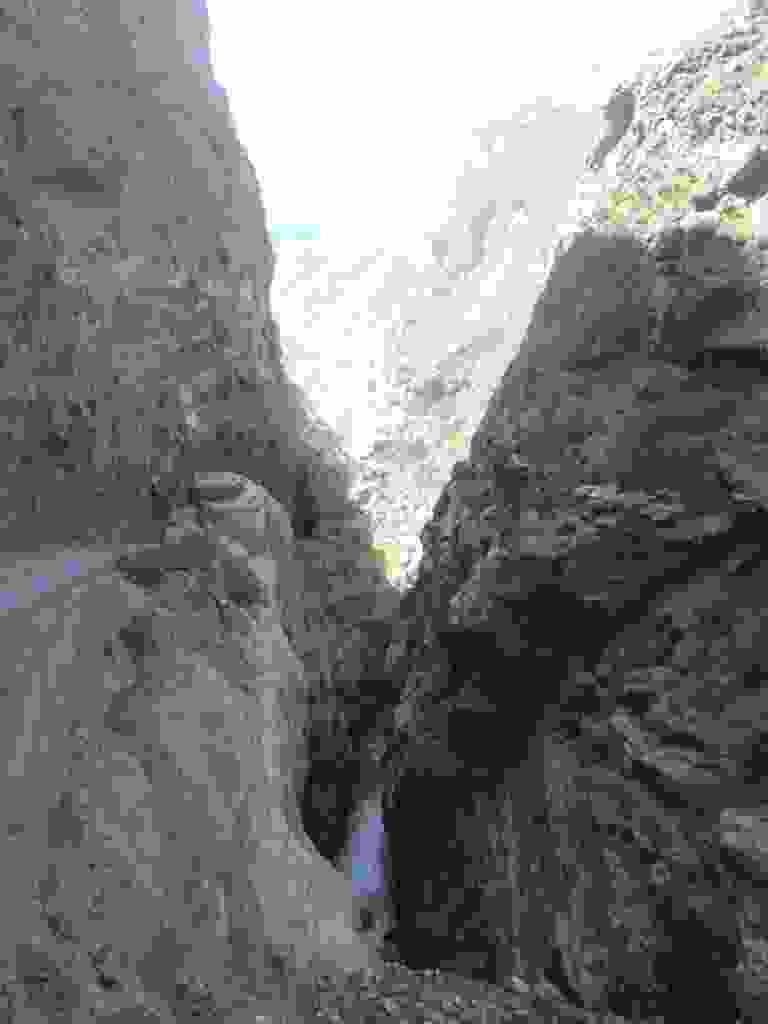
\includegraphics[width=0.6\textwidth]{../wp-content/uploads/2015/06/P6074761-768x1024.jpg} \end{center}
\begin{center} 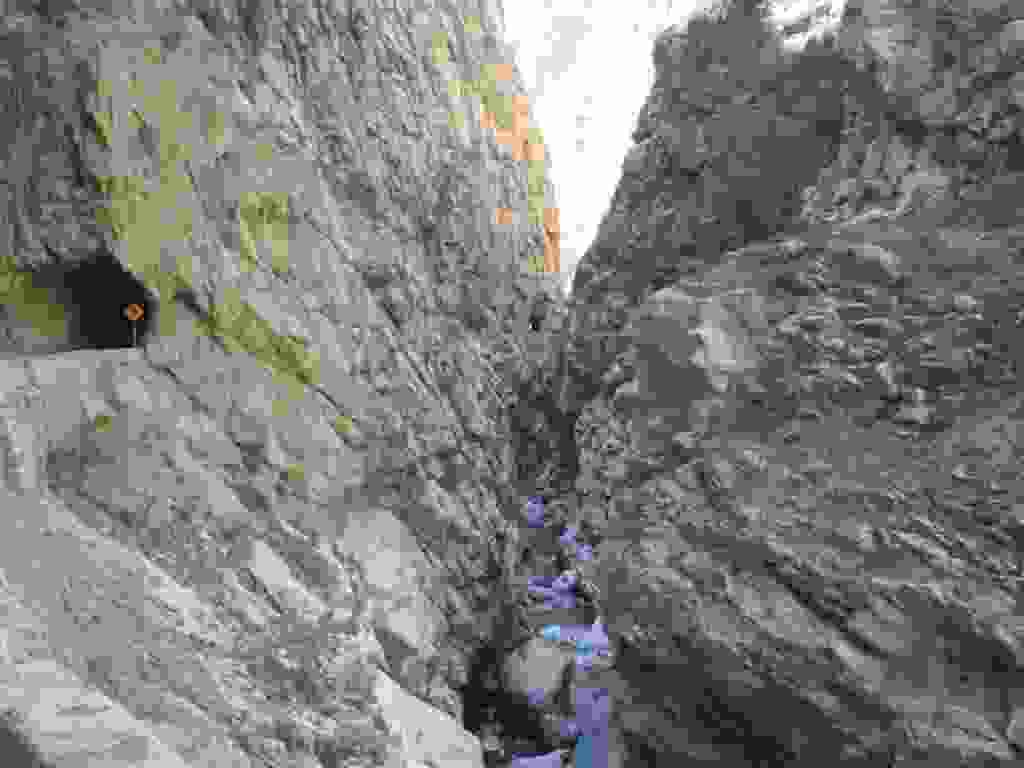
\includegraphics[width=\mywidth]{../wp-content/uploads/2015/06/P6074764-1024x768.jpg} \end{center}
\begin{center} 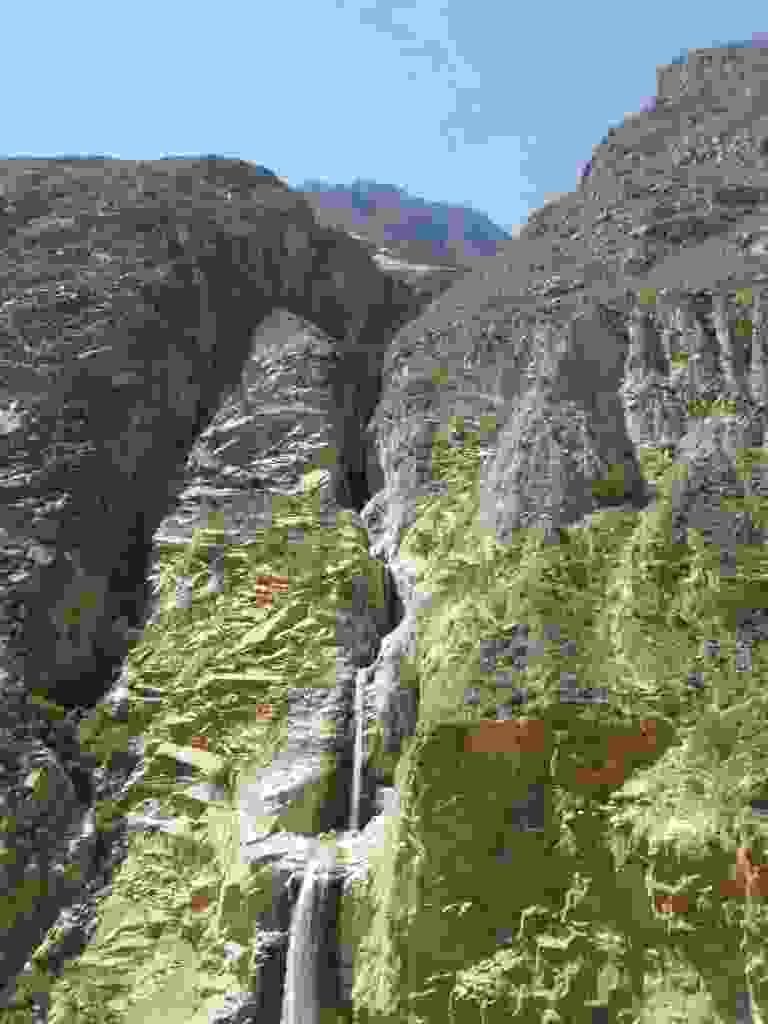
\includegraphics[width=0.6\textwidth]{../wp-content/uploads/2015/06/P6074766-768x1024.jpg} \end{center}
\begin{center} 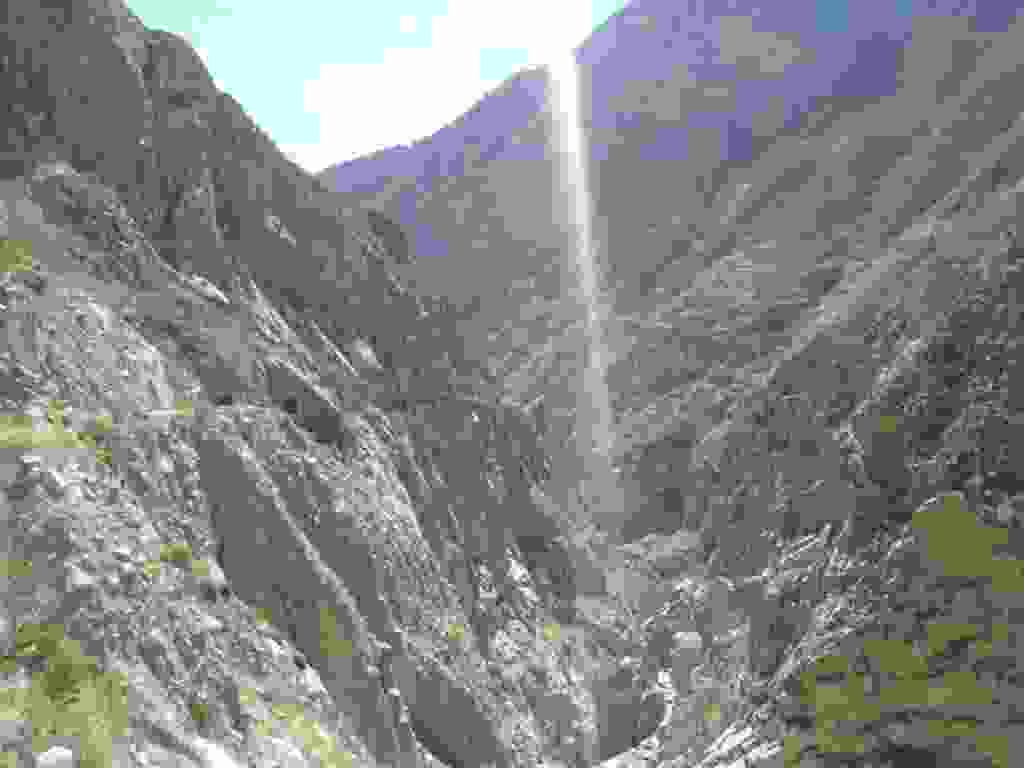
\includegraphics[width=\mywidth]{../wp-content/uploads/2015/06/P6074767-1024x768.jpg} \end{center}

\pagebreak
Puis je retrouve une piste non asphaltée, ça faisait un moment. 
\begin{center} 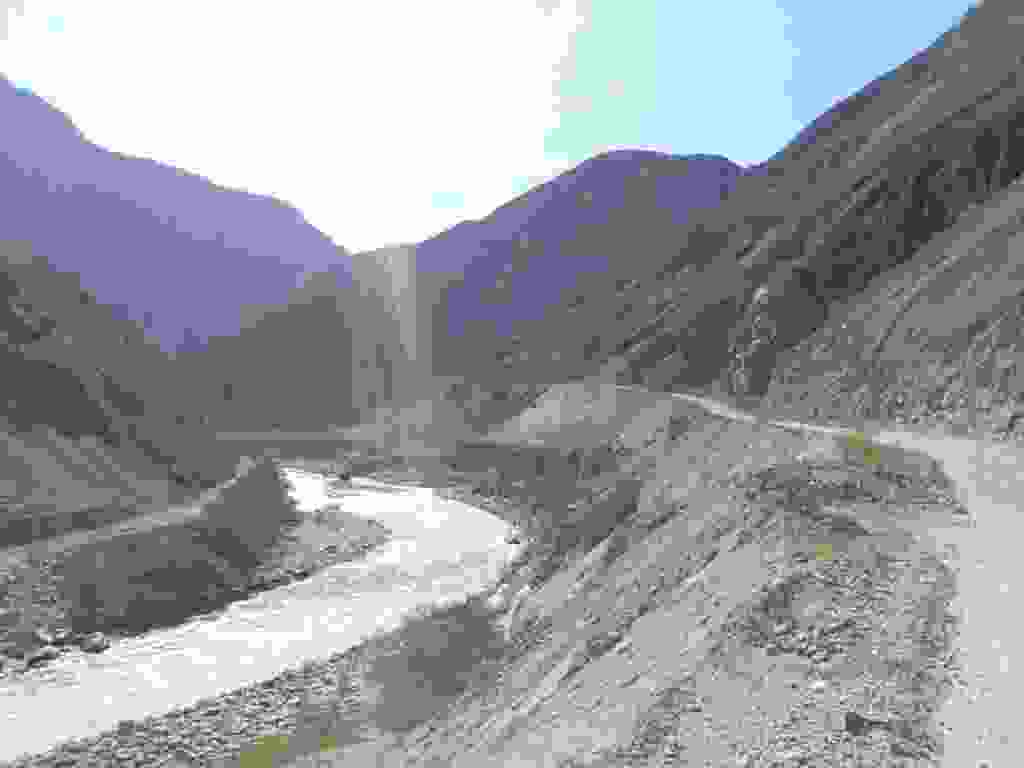
\includegraphics[width=\mywidth]{../wp-content/uploads/2015/06/P6074770-1024x768.jpg} \end{center}
\begin{center} 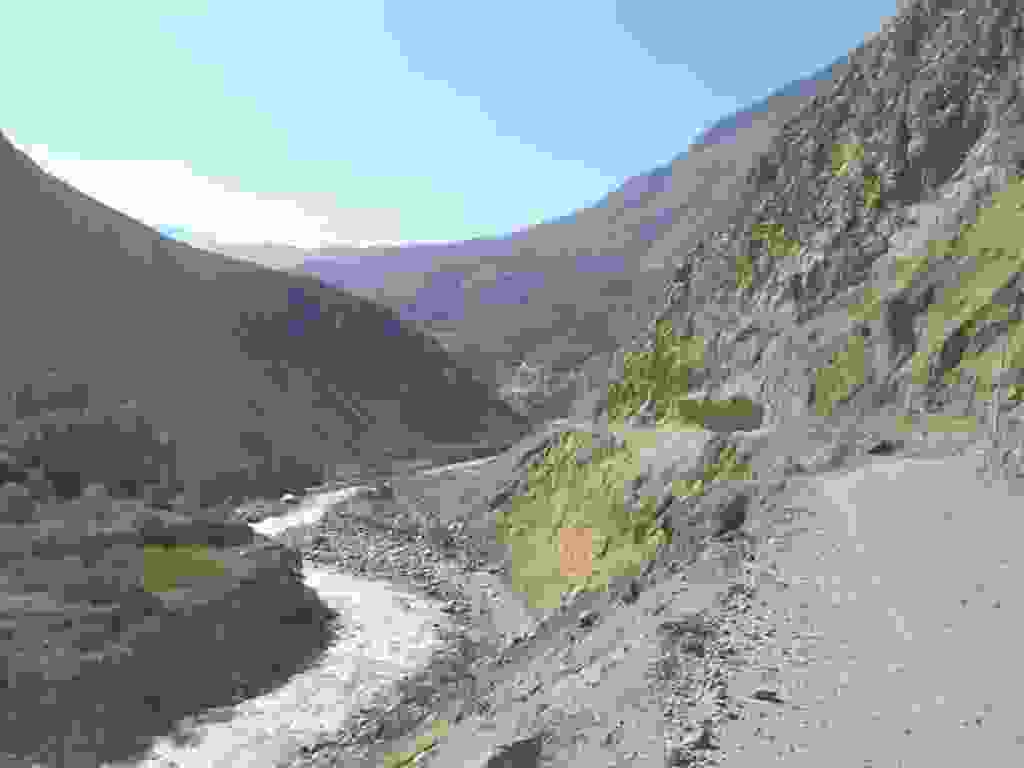
\includegraphics[width=\mywidth]{../wp-content/uploads/2015/06/P6074772-1024x768.jpg} \end{center}
\begin{center} 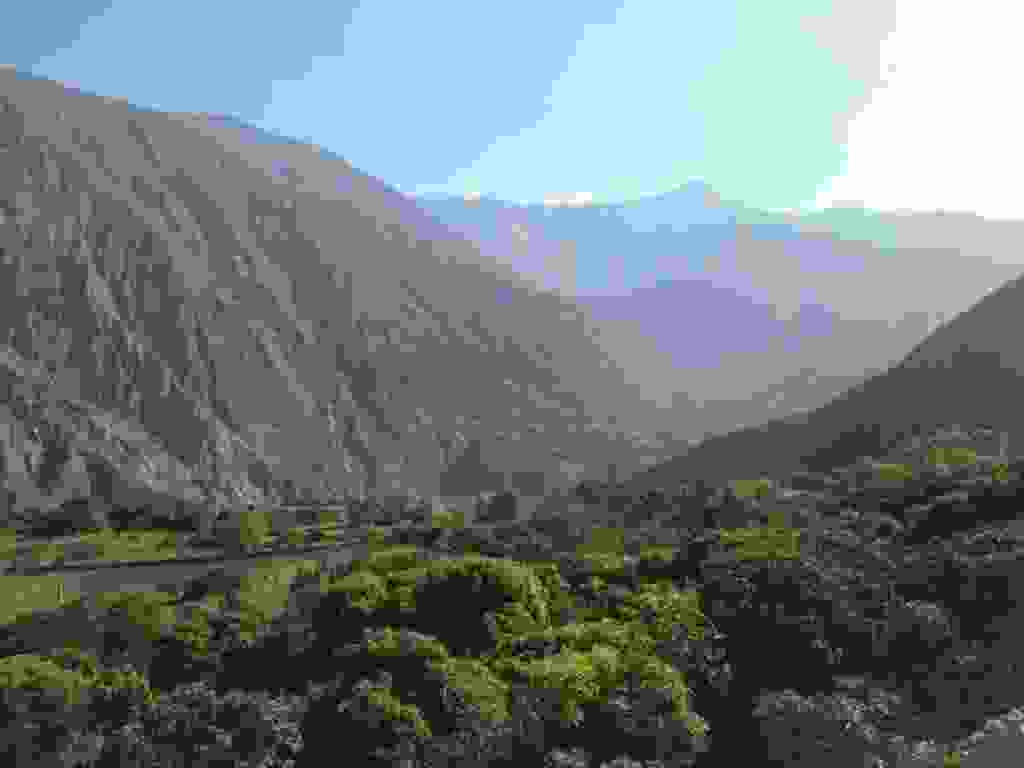
\includegraphics[width=\mywidth]{../wp-content/uploads/2015/06/P6074775-1024x768.jpg} \end{center}

Encore une portion bien encaissée. 
\begin{center} 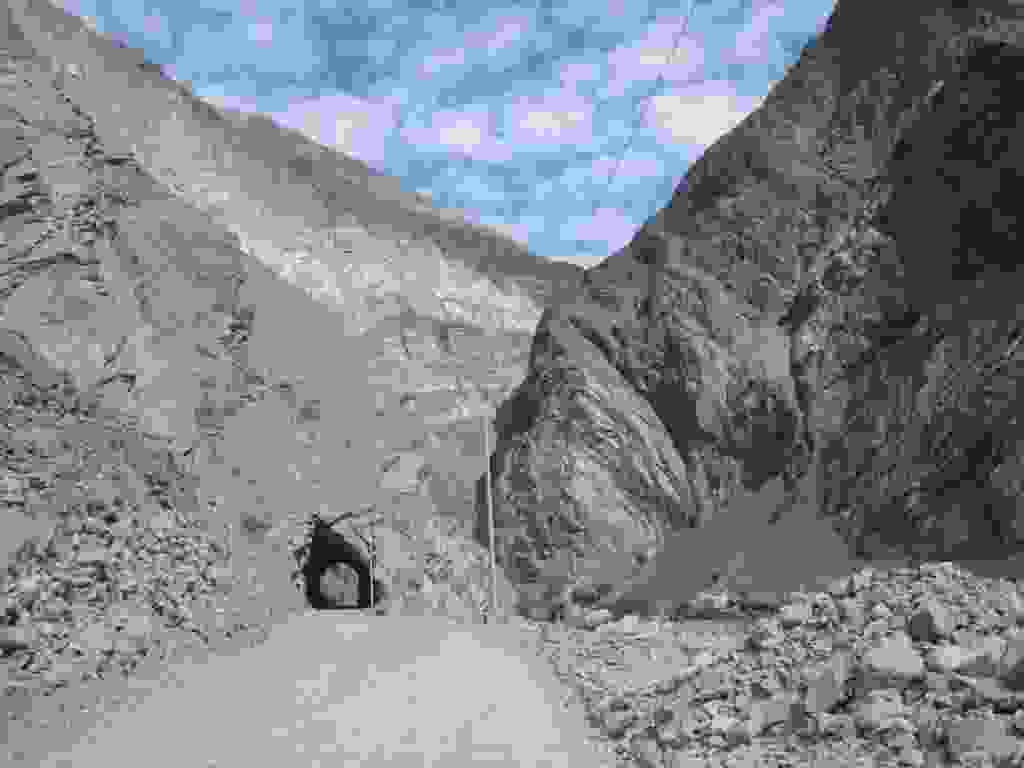
\includegraphics[width=\mywidth]{../wp-content/uploads/2015/06/P6084784-1024x768.jpg} \end{center}
\begin{center} 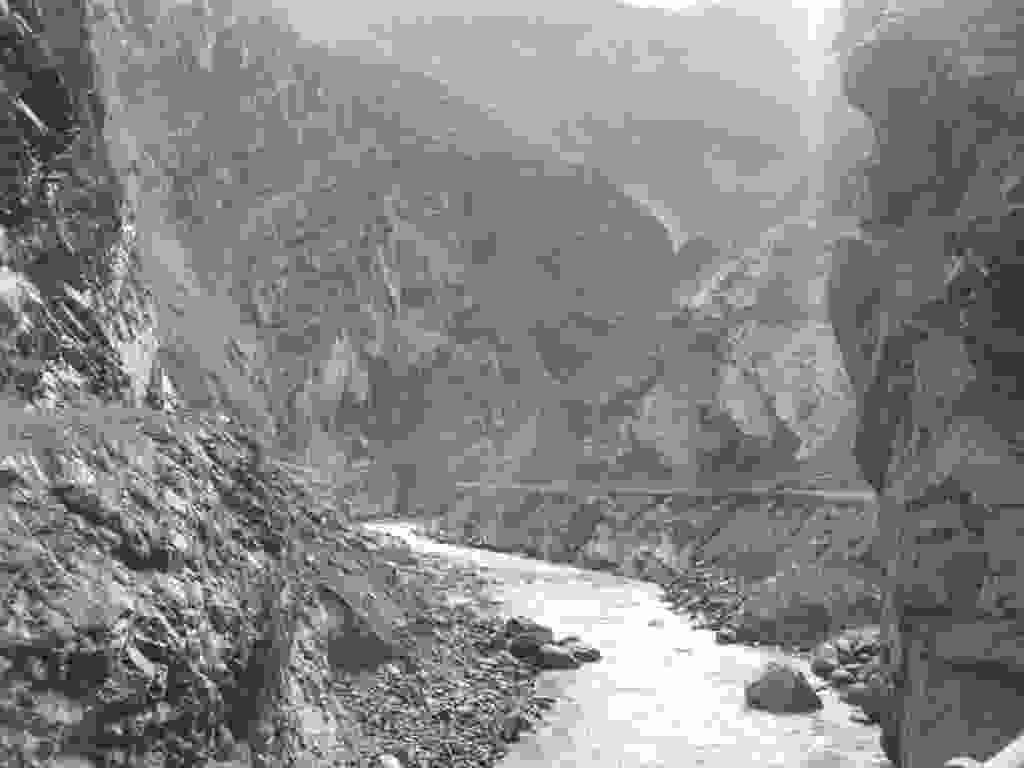
\includegraphics[width=\mywidth]{../wp-content/uploads/2015/06/P6084786-1024x768.jpg} \end{center}

Je traverse de rares villages qui paraissent quasiment abandonnés. Peu de possibilités de ravitaillement sur cette route, j'étais content d'avoir le filtre pour prendre de l'eau dans la riviere. 
\begin{center} 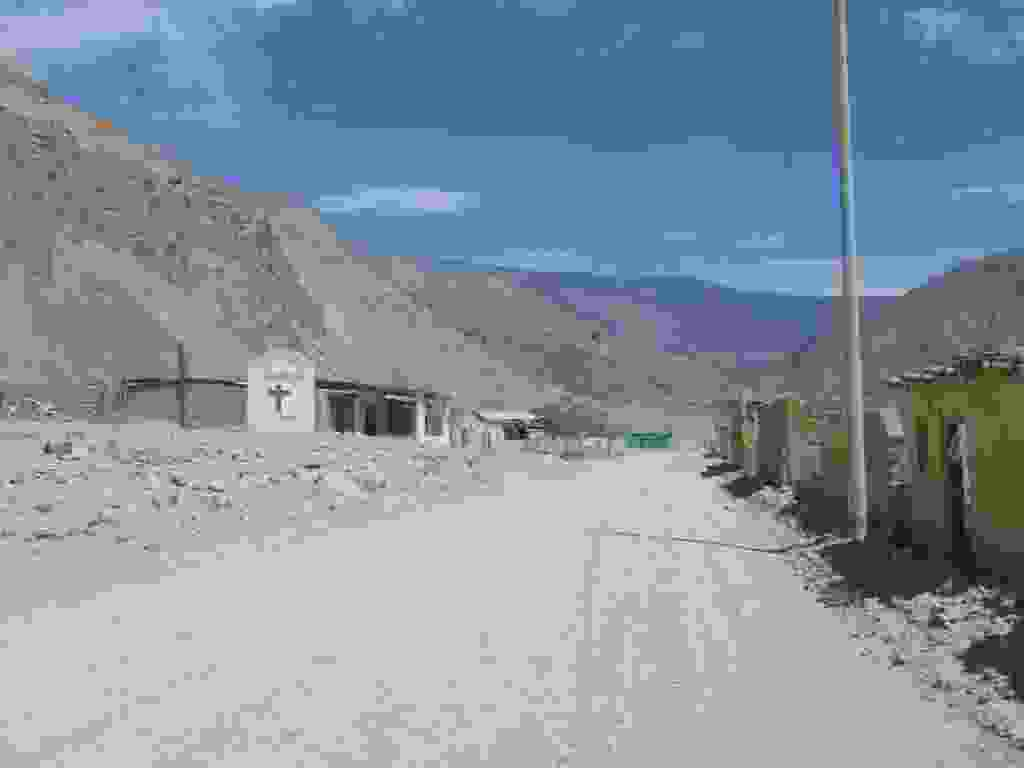
\includegraphics[width=\mywidth]{../wp-content/uploads/2015/06/P6084790-1024x768.jpg} \end{center}
\begin{center} 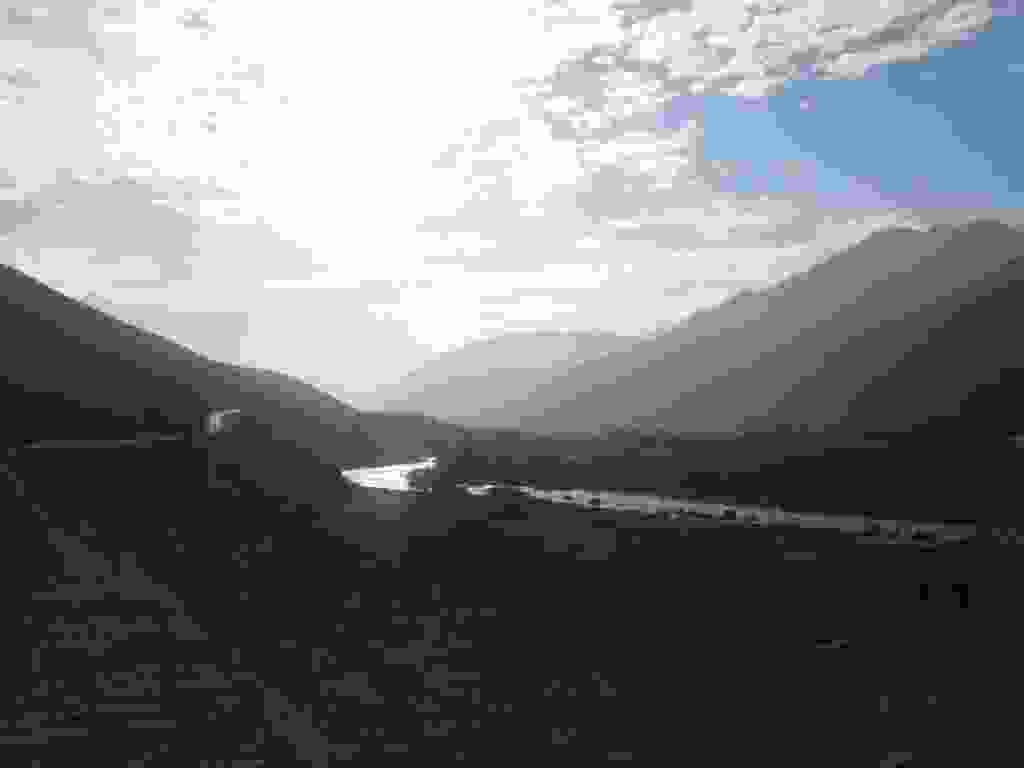
\includegraphics[width=\mywidth]{../wp-content/uploads/2015/06/P6094794-1024x768.jpg} \end{center}

J'arrive dans le désert quasiment au niveau de la mer. La chaleur est étouffante surtout avec la poussière de la piste. 
\begin{center} 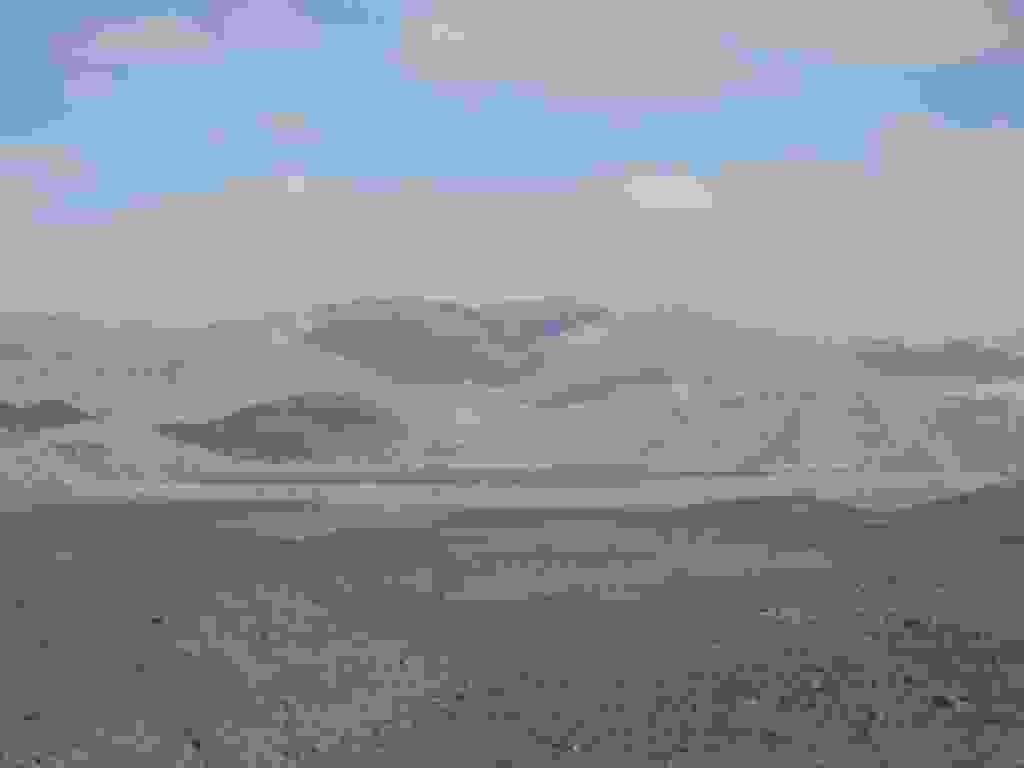
\includegraphics[width=\mywidth]{../wp-content/uploads/2015/06/P6094797-1024x768.jpg} \end{center}

\pagebreak
La dernière partie est sur la route panaméricaine. 
\begin{center} 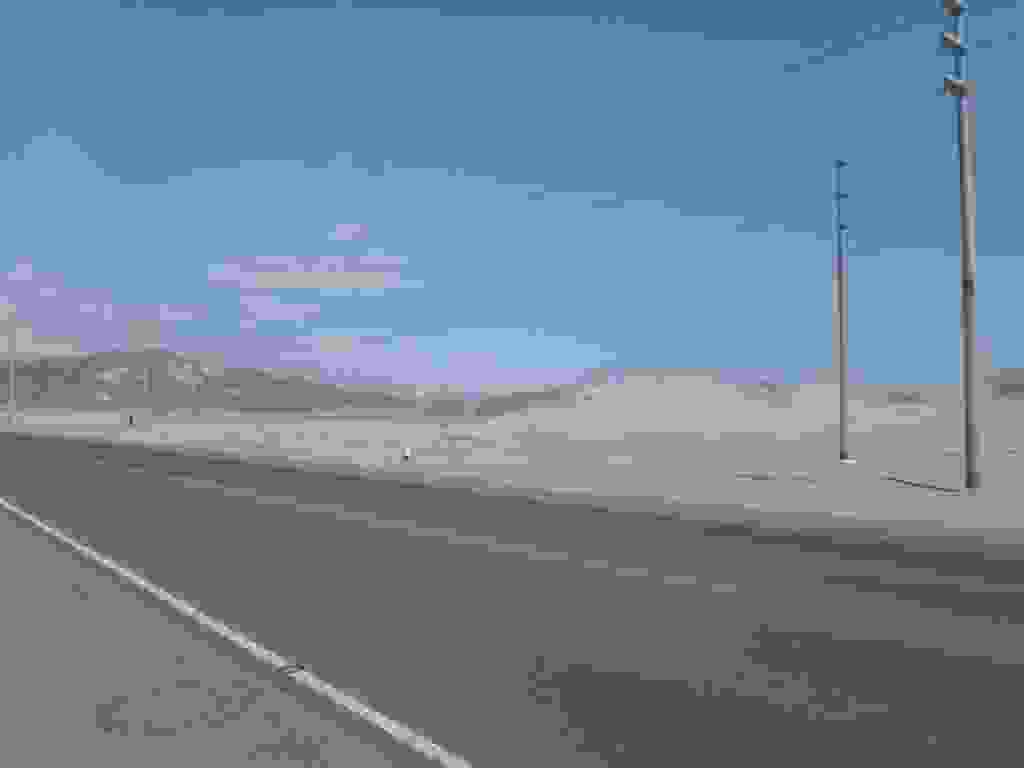
\includegraphics[width=\mywidth]{../wp-content/uploads/2015/06/P6094799-1024x768.jpg} \end{center}

Enfin, j'arrive à Trujillo où je retrouve une casa de ciclistas, la plus ancienne d'Amérique du Sud tenue par Lucho. Je rencontre 3 cyclistes français, 2 belges et un américain. 
\begin{center} 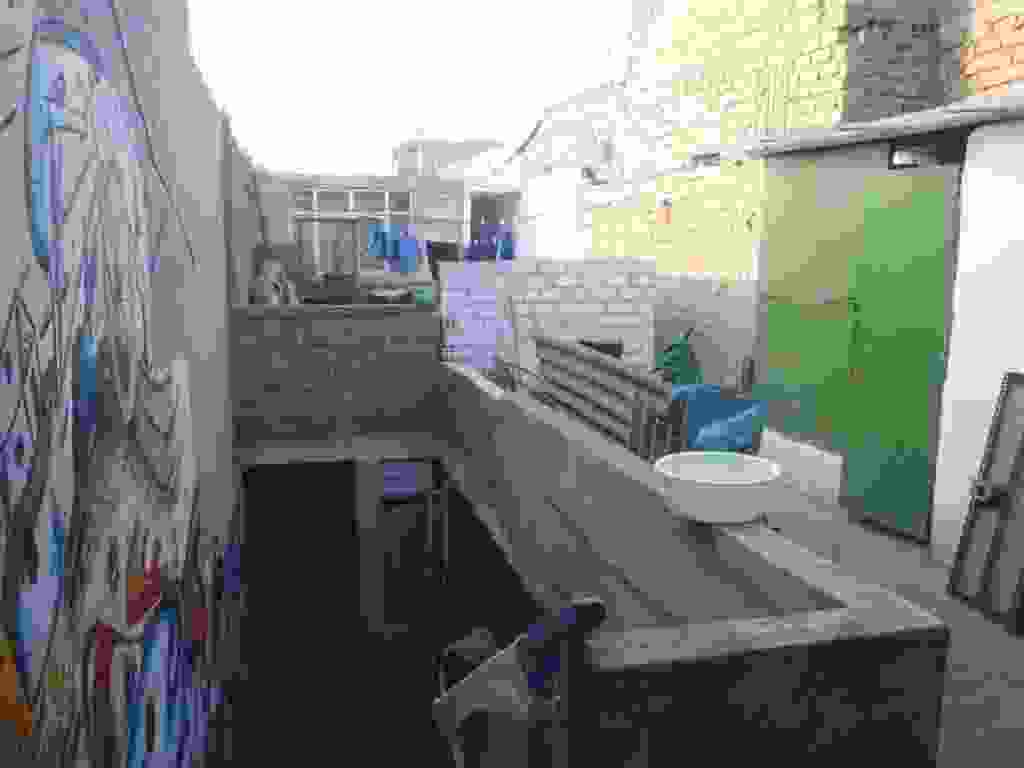
\includegraphics[width=\mywidth]{../wp-content/uploads/2015/06/P6114835-1024x768.jpg} \end{center}
\begin{center} 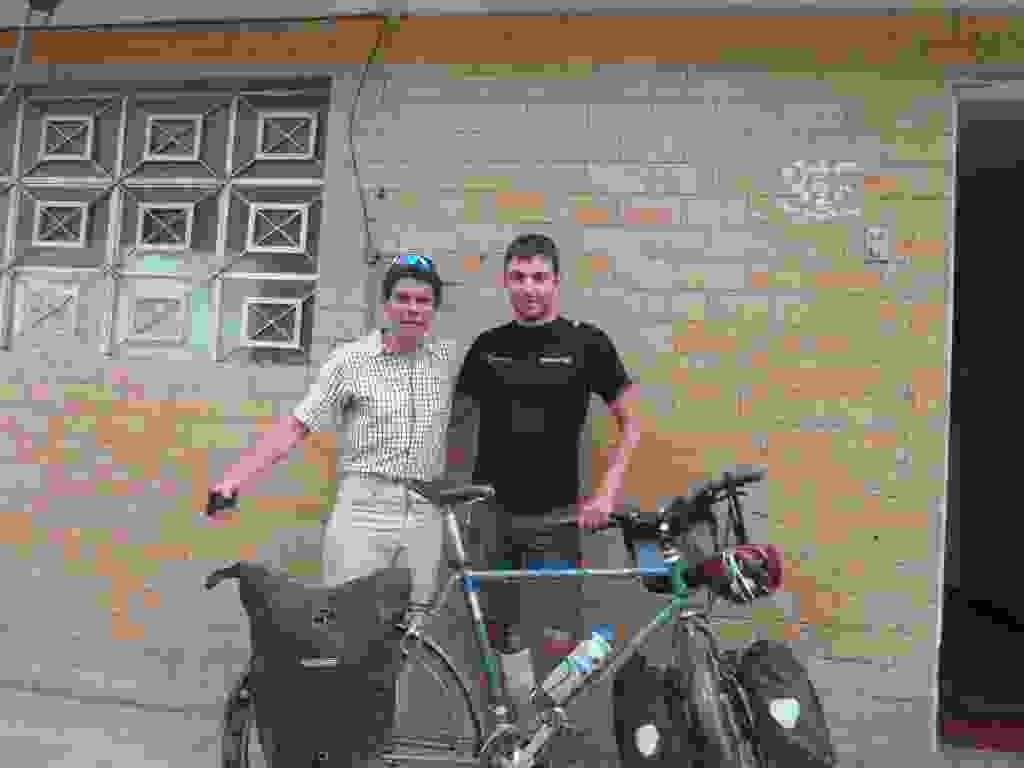
\includegraphics[width=\mywidth]{../wp-content/uploads/2015/06/P6114838-1024x768.jpg} \end{center}

La place d'armes de Trujillo. 
\begin{center} 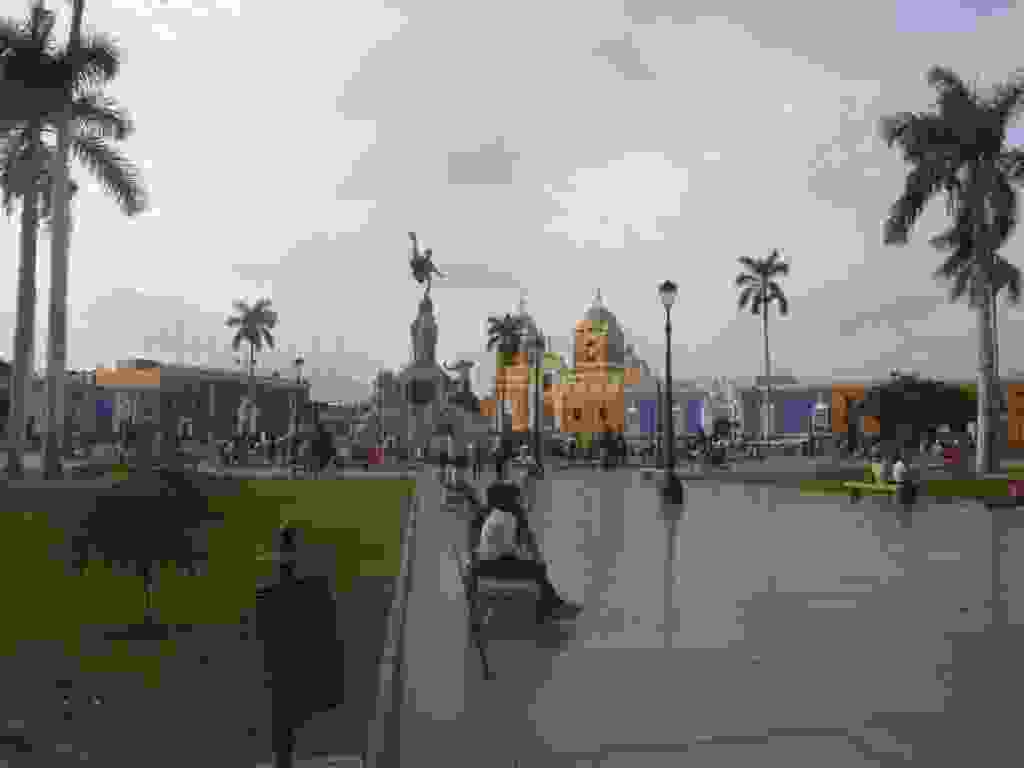
\includegraphics[width=\mywidth]{../wp-content/uploads/2015/06/P6104806-1024x768.jpg} \end{center}

\pagebreak
Les ruines de Chan Chan à quelques km, une cité pré inca construite tout en terre. 
\begin{center} 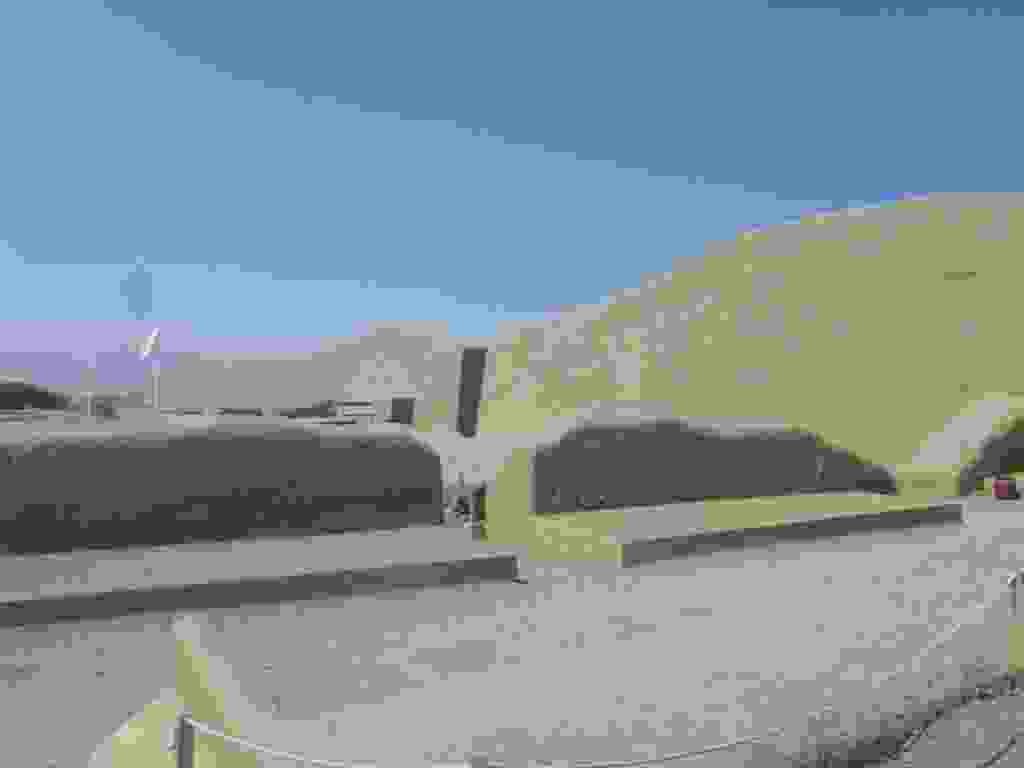
\includegraphics[width=\mywidth]{../wp-content/uploads/2015/06/P6104824-1024x768.jpg} \end{center}
\begin{center} 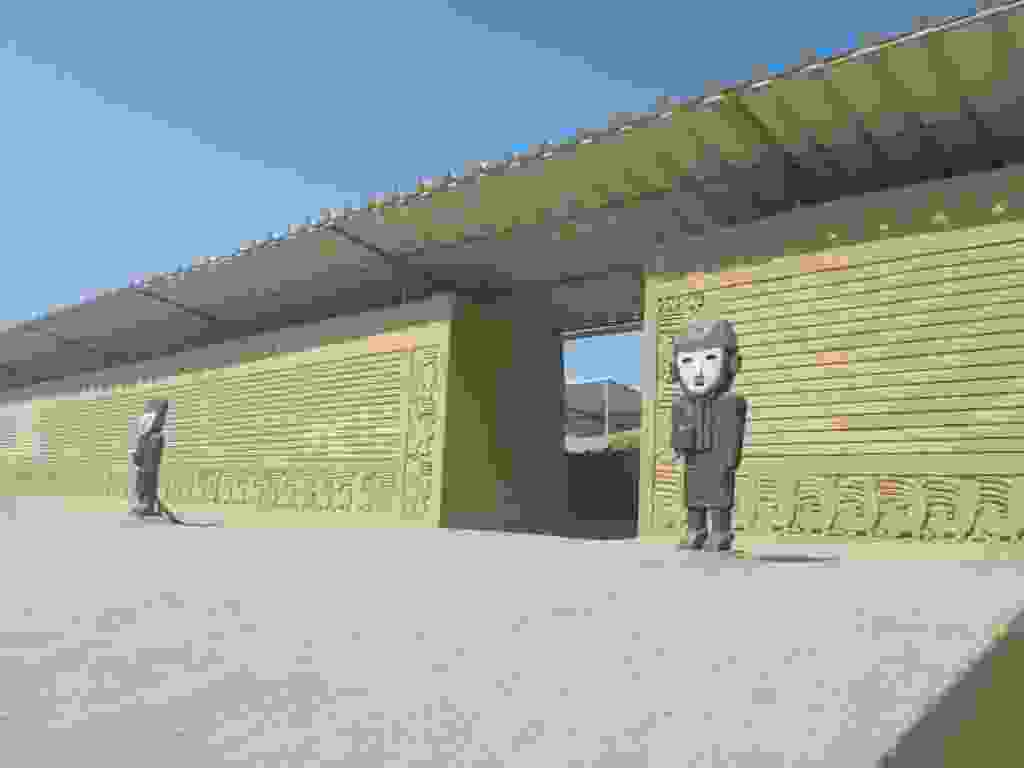
\includegraphics[width=\mywidth]{../wp-content/uploads/2015/06/P6104808-1024x768.jpg} \end{center}
\begin{center} 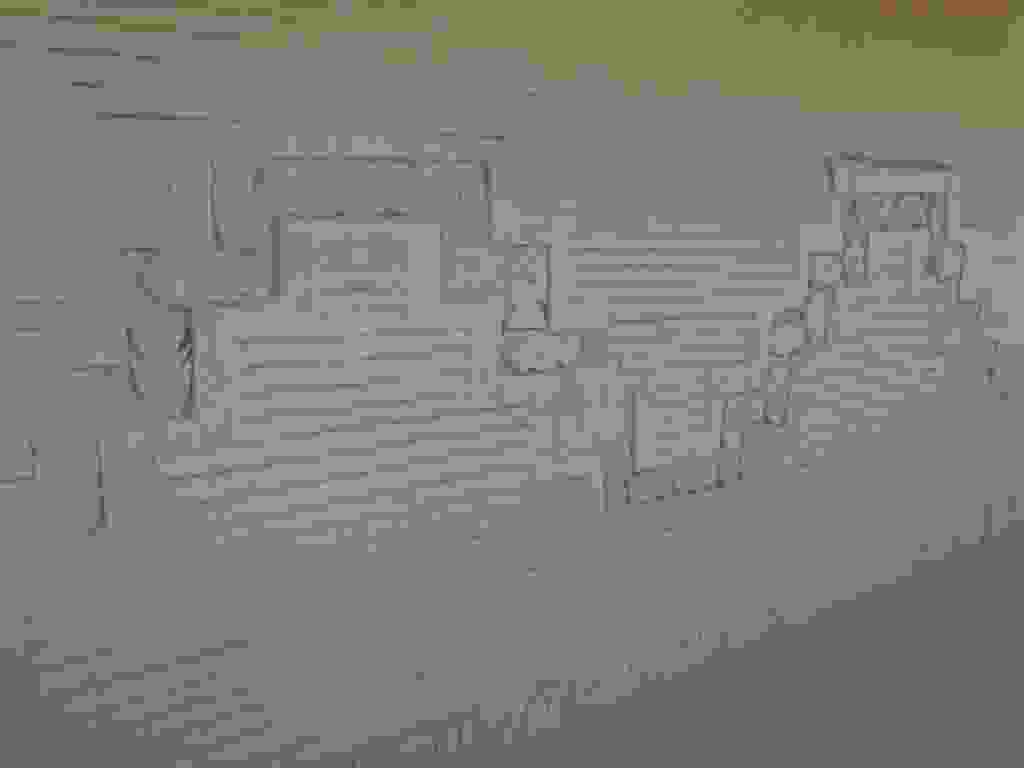
\includegraphics[width=\mywidth]{../wp-content/uploads/2015/06/P6104810-1024x768.jpg} \end{center}
\begin{center} 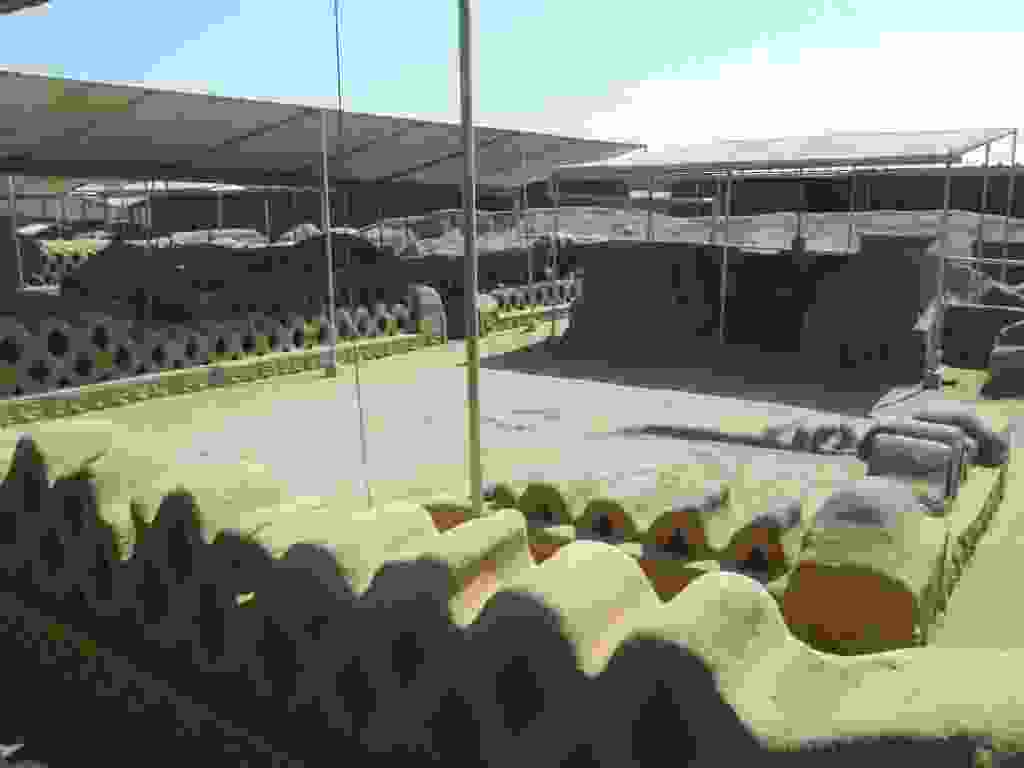
\includegraphics[width=\mywidth]{../wp-content/uploads/2015/06/P6104815-1024x768.jpg} \end{center}

\pagebreak
La station balnéaire de Huanchaco au bord du Pacifique : beaucoup de surfeurs et des pécheurs sur leurs embarcations en roseau. J'y ai croisé par hasard Jan avec qui j'avais fait le trek du Salkantay. 
\begin{center} 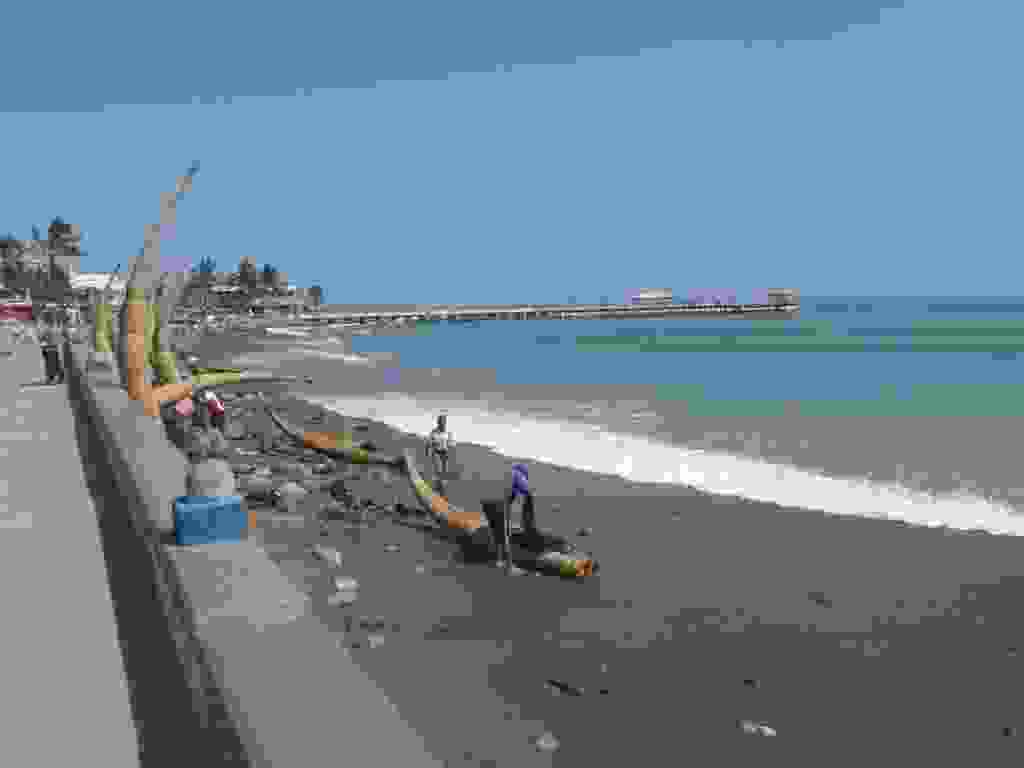
\includegraphics[width=\mywidth]{../wp-content/uploads/2015/06/P6104830-1024x768.jpg} \end{center}
\begin{center} 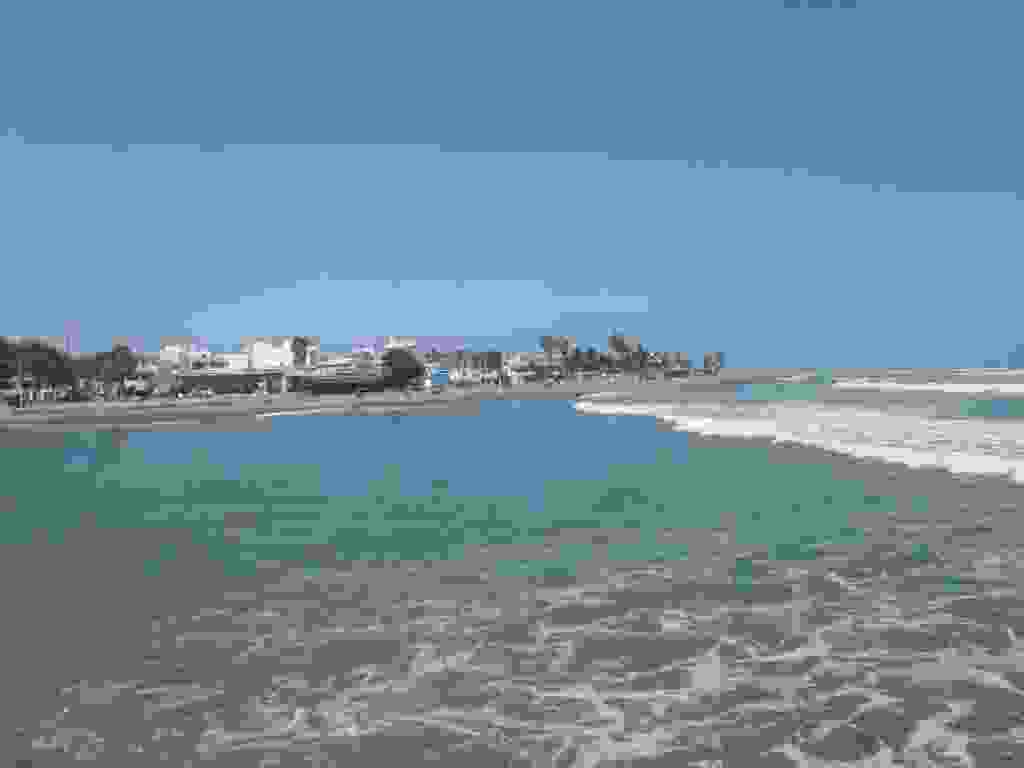
\includegraphics[width=\mywidth]{../wp-content/uploads/2015/06/P6104827-1024x768.jpg} \end{center}

\`A bientôt en Équateur !